% Options for packages loaded elsewhere
\PassOptionsToPackage{unicode}{hyperref}
\PassOptionsToPackage{hyphens}{url}
%
\documentclass[
]{article}
\usepackage{amsmath,amssymb}
\usepackage{iftex}
\ifPDFTeX
  \usepackage[T1]{fontenc}
  \usepackage[utf8]{inputenc}
  \usepackage{textcomp} % provide euro and other symbols
\else % if luatex or xetex
  \usepackage{unicode-math} % this also loads fontspec
  \defaultfontfeatures{Scale=MatchLowercase}
  \defaultfontfeatures[\rmfamily]{Ligatures=TeX,Scale=1}
\fi
\usepackage{lmodern}
\ifPDFTeX\else
  % xetex/luatex font selection
\fi
% Use upquote if available, for straight quotes in verbatim environments
\IfFileExists{upquote.sty}{\usepackage{upquote}}{}
\IfFileExists{microtype.sty}{% use microtype if available
  \usepackage[]{microtype}
  \UseMicrotypeSet[protrusion]{basicmath} % disable protrusion for tt fonts
}{}
\makeatletter
\@ifundefined{KOMAClassName}{% if non-KOMA class
  \IfFileExists{parskip.sty}{%
    \usepackage{parskip}
  }{% else
    \setlength{\parindent}{0pt}
    \setlength{\parskip}{6pt plus 2pt minus 1pt}}
}{% if KOMA class
  \KOMAoptions{parskip=half}}
\makeatother
\usepackage{xcolor}
\usepackage[margin=1in]{geometry}
\usepackage{longtable,booktabs,array}
\usepackage{calc} % for calculating minipage widths
% Correct order of tables after \paragraph or \subparagraph
\usepackage{etoolbox}
\makeatletter
\patchcmd\longtable{\par}{\if@noskipsec\mbox{}\fi\par}{}{}
\makeatother
% Allow footnotes in longtable head/foot
\IfFileExists{footnotehyper.sty}{\usepackage{footnotehyper}}{\usepackage{footnote}}
\makesavenoteenv{longtable}
\usepackage{graphicx}
\makeatletter
\def\maxwidth{\ifdim\Gin@nat@width>\linewidth\linewidth\else\Gin@nat@width\fi}
\def\maxheight{\ifdim\Gin@nat@height>\textheight\textheight\else\Gin@nat@height\fi}
\makeatother
% Scale images if necessary, so that they will not overflow the page
% margins by default, and it is still possible to overwrite the defaults
% using explicit options in \includegraphics[width, height, ...]{}
\setkeys{Gin}{width=\maxwidth,height=\maxheight,keepaspectratio}
% Set default figure placement to htbp
\makeatletter
\def\fps@figure{htbp}
\makeatother
\setlength{\emergencystretch}{3em} % prevent overfull lines
\providecommand{\tightlist}{%
  \setlength{\itemsep}{0pt}\setlength{\parskip}{0pt}}
\setcounter{secnumdepth}{-\maxdimen} % remove section numbering
\ifLuaTeX
  \usepackage{selnolig}  % disable illegal ligatures
\fi
\usepackage{bookmark}
\IfFileExists{xurl.sty}{\usepackage{xurl}}{} % add URL line breaks if available
\urlstyle{same}
\hypersetup{
  pdftitle={Actividad2 Unidad 2 InformeEjecutivo},
  pdfauthor={Juan José Restrepo Rosero},
  hidelinks,
  pdfcreator={LaTeX via pandoc}}

\title{Actividad2 Unidad 2 InformeEjecutivo}
\author{Juan José Restrepo Rosero}
\date{2025-03-03}

\begin{document}
\maketitle

{
\setcounter{tocdepth}{2}
\tableofcontents
}
\section{\texorpdfstring{\textbf{Caso C\&A}}{Caso C\&A}}\label{caso-ca}

\subsection{\texorpdfstring{\textbf{Enunciado}}{Enunciado}}\label{enunciado}

Maria comenzó como agente de bienes raíces en Cali hace 10 años. Después
de laborar dos años para una empresa nacional, se traslado a Bogotá y
trabajó para otra agencia de bienes raíces. Sus amigos y familiares la
convencieron de que con su experiencia y conocimientos del negocio debía
abrir su propia agencia. Terminó por adquirir la licencia de
intermediario y al poco tiempo fundó su propia compañía, C\&A (Casas y
Apartamentos) en Cali. Santiago y Lina, dos vendedores de la empresa
anterior aceptaron trabajar en la nueva compaña. En la actualidad ocho
agentes de bienes raíces colaboran con ella en C\&A.

Actualmente las ventas de bienes raíces en Cali se han visto disminuidas
de manera significativa en lo corrido del año. Durante este periodo
muchas instituciones bancarias de ahorro y vivienda están prestando
grandes sumas de dinero para la industria y la construcción comercial y
residencial. Cuando el efecto producto de las tensiones políticas y
sociales disminuya, se espera que la actividad económica de este sector
se reactive.

Hace dos días, María recibió una carta solicitando asesoría para la
compra de dos viviendas por parte de una compañía internacional que
desea ubicar a dos de sus empleados con sus familias en la ciudad. Las
solicitudes incluyen las siguientes condiciones:

\begin{figure}
\centering
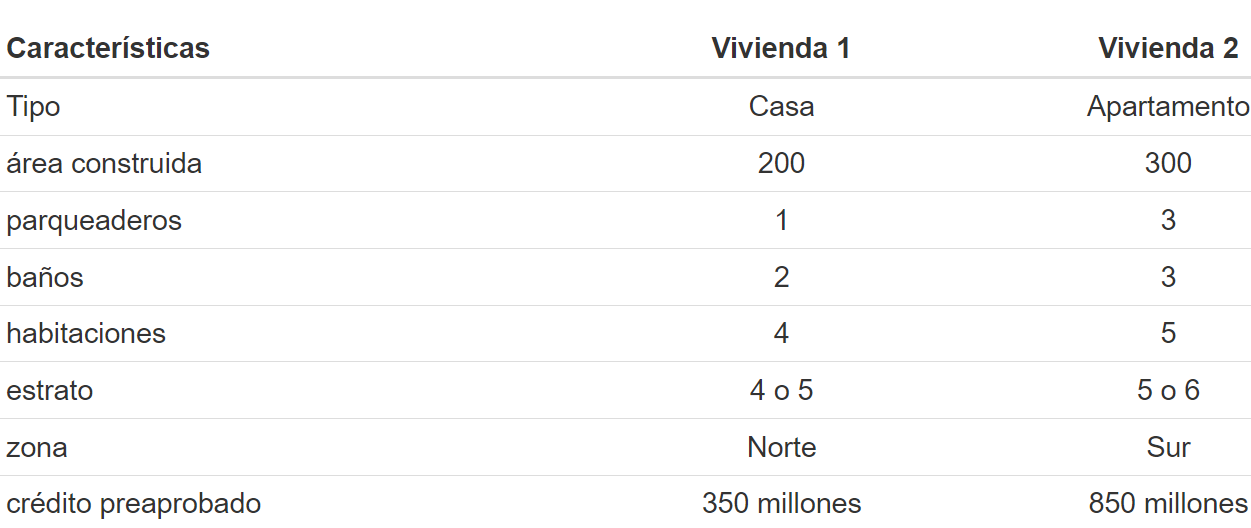
\includegraphics{C:/Users/Juan Jose Restrepo/Desktop/Master-Data-Science-main/Semestre 2/Modelos Estadisticos/A2_U2_InformeEjecutivo_JJRR/condiciones.png}
\caption{Condiciones de las solicitudes}
\end{figure}

\subsection{\texorpdfstring{\textbf{Pasos requeridos para la obtención
de los
resultados}}{Pasos requeridos para la obtención de los resultados}}\label{pasos-requeridos-para-la-obtenciuxf3n-de-los-resultados}

\begin{enumerate}
\def\labelenumi{\arabic{enumi}.}
\item
  Realice un filtro a la base de datos e incluya solo las ofertas de:
  base1: casas, de la zona norte de la ciudad. Presente los primeros 3
  registros de las bases y algunas tablas que comprueben la consulta.
  (Adicional un mapa con los puntos de las bases. Discutir si todos los
  puntos se ubican en la zona correspondiente o se presentan valores en
  otras zonas, por qué?).
\item
  Realice un análisis exploratorio de datos enfocado en la correlación
  entre la variable respuesta (precio de la casa) en función del área
  construida, estrato, número de baños, número de habitaciones y zona
  donde se ubica la vivienda. Use gráficos interactivos con el paquete
  plotly e interprete los resultados.
\item
  Estime un modelo de regresión lineal múltiple con las variables del
  punto anterior (precio = f(área construida, estrato, número de
  cuartos, número de parqueaderos, número de baños)) e interprete los
  coeficientes si son estadísticamente significativos. Las
  interpretaciones deben estar contextualizadas y discutir si los
  resultados son lógicos. Adicionalmente interprete el coeficiente
  \(R^2\) y discuta el ajuste del modelo e implicaciones (qué podrían
  hacer para mejorarlo).
\item
  Realice la validación de supuestos del modelo e interprete los
  resultados (no es necesario corregir en caso de presentar problemas,
  solo realizar sugerencias de qué se podría hacer).
\item
  Con el modelo identificado debe predecir el precio de la vivienda con
  las características de la primera solicitud.
\item
  Con las predicciones del modelo sugiera potenciales ofertas que
  respondan a la solicitud de la vivienda 1. Tenga en cuenta que la
  empresa tiene crédito pre-aprobado de máximo 350 millones de pesos.
  Realice un análisis y presente en un mapa al menos 5 ofertas
  potenciales que debe discutir.
\item
  Realice los pasos del \textbf{1} al \textbf{6} para la segunda
  solicitud que tiene un crédito pre-aprobado por valor de \$850
  millones.
\end{enumerate}

\subsection{\texorpdfstring{\textbf{Exploración inicial de
datos}}{Exploración inicial de datos}}\label{exploraciuxf3n-inicial-de-datos}

En base al resumen y la estructura del conjunto de datos, se pueden
destacar varios puntos importantes. El dataset contiene
\textbf{\emph{8322}} registros distribuidos en 13 variables. Se observa
que algunas variables, como piso, estrato, preciom, areaconst,
parqueaderos, banios, habitaciones, longitud y latitud, presentan
valores ausentes, lo cual indica la necesidad de tratar dichos vacíos
antes de realizar análisis posteriores.

Mientras que las variables \textbf{\emph{zona, piso, tipo y barrio}} son
de carácter categórico, las variables \textbf{\emph{id, estrato,
preciom, areaconst, parqueaderos, banios, habitaciones, longitud y
latitud}} son numéricas. Además, se han detectado posibles
inconsistencias o errores en los datos que requieren atención durante el
proceso de análisis.

En resumen, este conjunto de datos ofrece información diversa sobre
propiedades inmobiliarias, incluyendo aspectos de ubicación,
características y precios, pero necesitará un procesamiento cuidadoso
para asegurar su validez y utilidad en estudios futuros.

\begin{verbatim}
##        id           zona               piso              estrato     
##  Min.   :   1   Length:8322        Length:8322        Min.   :3.000  
##  1st Qu.:2080   Class :character   Class :character   1st Qu.:4.000  
##  Median :4160   Mode  :character   Mode  :character   Median :5.000  
##  Mean   :4160                                         Mean   :4.634  
##  3rd Qu.:6240                                         3rd Qu.:5.000  
##  Max.   :8319                                         Max.   :6.000  
##  NA's   :3                                            NA's   :3      
##     preciom         areaconst       parqueaderos        banios      
##  Min.   :  58.0   Min.   :  30.0   Min.   : 1.000   Min.   : 0.000  
##  1st Qu.: 220.0   1st Qu.:  80.0   1st Qu.: 1.000   1st Qu.: 2.000  
##  Median : 330.0   Median : 123.0   Median : 2.000   Median : 3.000  
##  Mean   : 433.9   Mean   : 174.9   Mean   : 1.835   Mean   : 3.111  
##  3rd Qu.: 540.0   3rd Qu.: 229.0   3rd Qu.: 2.000   3rd Qu.: 4.000  
##  Max.   :1999.0   Max.   :1745.0   Max.   :10.000   Max.   :10.000  
##  NA's   :2        NA's   :3        NA's   :1605     NA's   :3       
##   habitaciones        tipo              barrio             longitud     
##  Min.   : 0.000   Length:8322        Length:8322        Min.   :-76.59  
##  1st Qu.: 3.000   Class :character   Class :character   1st Qu.:-76.54  
##  Median : 3.000   Mode  :character   Mode  :character   Median :-76.53  
##  Mean   : 3.605                                         Mean   :-76.53  
##  3rd Qu.: 4.000                                         3rd Qu.:-76.52  
##  Max.   :10.000                                         Max.   :-76.46  
##  NA's   :3                                              NA's   :3       
##     latitud     
##  Min.   :3.333  
##  1st Qu.:3.381  
##  Median :3.416  
##  Mean   :3.418  
##  3rd Qu.:3.452  
##  Max.   :3.498  
##  NA's   :3
\end{verbatim}

\begin{verbatim}
## spc_tbl_ [8,322 x 13] (S3: spec_tbl_df/tbl_df/tbl/data.frame)
##  $ id          : num [1:8322] 1147 1169 1350 5992 1212 ...
##  $ zona        : chr [1:8322] "Zona Oriente" "Zona Oriente" "Zona Oriente" "Zona Sur" ...
##  $ piso        : chr [1:8322] NA NA NA "02" ...
##  $ estrato     : num [1:8322] 3 3 3 4 5 5 4 5 5 5 ...
##  $ preciom     : num [1:8322] 250 320 350 400 260 240 220 310 320 780 ...
##  $ areaconst   : num [1:8322] 70 120 220 280 90 87 52 137 150 380 ...
##  $ parqueaderos: num [1:8322] 1 1 2 3 1 1 2 2 2 2 ...
##  $ banios      : num [1:8322] 3 2 2 5 2 3 2 3 4 3 ...
##  $ habitaciones: num [1:8322] 6 3 4 3 3 3 3 4 6 3 ...
##  $ tipo        : chr [1:8322] "Casa" "Casa" "Casa" "Casa" ...
##  $ barrio      : chr [1:8322] "20 de julio" "20 de julio" "20 de julio" "3 de julio" ...
##  $ longitud    : num [1:8322] -76.5 -76.5 -76.5 -76.5 -76.5 ...
##  $ latitud     : num [1:8322] 3.43 3.43 3.44 3.44 3.46 ...
##  - attr(*, "spec")=
##   .. cols(
##   ..   id = col_double(),
##   ..   zona = col_character(),
##   ..   piso = col_character(),
##   ..   estrato = col_double(),
##   ..   preciom = col_double(),
##   ..   areaconst = col_double(),
##   ..   parqueaderos = col_double(),
##   ..   banios = col_double(),
##   ..   habitaciones = col_double(),
##   ..   tipo = col_character(),
##   ..   barrio = col_character(),
##   ..   longitud = col_double(),
##   ..   latitud = col_double()
##   .. )
##  - attr(*, "problems")=<externalptr>
\end{verbatim}

\subsection{\texorpdfstring{\textbf{1. Realice un filtro a la base de
datos
}}{1. Realice un filtro a la base de datos }}\label{realice-un-filtro-a-la-base-de-datos}

\subsubsection{\texorpdfstring{\textbf{Base 1: Casas en Zona
Norte}}{Base 1: Casas en Zona Norte}}\label{base-1-casas-en-zona-norte}

De acuerdo con los requerimientos del informe, se ha generado un
subconjunto de datos enfocado exclusivamente en las ofertas de casas
ubicadas en la zona norte. Este subconjunto presenta las siguientes
características relevantes:

\begin{enumerate}
\def\labelenumi{\arabic{enumi}.}
\item
  \textbf{Diversidad y Completitud de Registros:}\\
  Se han extraído 722 registros, lo que evidencia una alta diversidad en
  las propiedades listadas. El proceso de filtrado ha sido eficaz para
  capturar únicamente aquellas casas situadas en la zona norte. Cabe
  señalar que se detectan algunos valores faltantes, lo cual es
  coherente con la estructura del dataset original.
\item
  \textbf{Amplio Rango en los Precios:}\\
  Los precios de las propiedades varían considerablemente, abarcando
  desde 58 hasta 1999 unidades monetarias. La mediana se sitúa cerca de
  390, mientras que la media es de aproximadamente 445.9, lo que sugiere
  que la mayoría de las ofertas se agrupan en torno a estos valores,
  reflejando la heterogeneidad del mercado.
\item
  \textbf{Variabilidad en el Área Construida:}\\
  El área construida de las viviendas oscila entre 30 y 1745 metros
  cuadrados. Los valores centrales, con una mediana alrededor de 240 y
  una media de cerca de 264.9, indican que la mayoría de las casas
  tienen dimensiones que se agrupan en este rango, ofreciendo una idea
  clara de la distribución de tamaños.
\item
  \textbf{Diversidad en Otros Atributos:}\\
  Otros indicadores importantes, como el número de parqueaderos, baños y
  habitaciones, también muestran una dispersión significativa,
  alcanzando en ocasiones un máximo de 10. Estos atributos son
  esenciales para comprender en detalle las características y el nivel
  de confort de las casas en la zona norte.
\end{enumerate}

\begin{verbatim}
## Primeros 3 registros de la base de datos filtrada:
\end{verbatim}

\begin{longtable}[]{@{}
  >{\raggedleft\arraybackslash}p{(\columnwidth - 24\tabcolsep) * \real{0.0455}}
  >{\raggedright\arraybackslash}p{(\columnwidth - 24\tabcolsep) * \real{0.1000}}
  >{\raggedright\arraybackslash}p{(\columnwidth - 24\tabcolsep) * \real{0.0455}}
  >{\raggedleft\arraybackslash}p{(\columnwidth - 24\tabcolsep) * \real{0.0727}}
  >{\raggedleft\arraybackslash}p{(\columnwidth - 24\tabcolsep) * \real{0.0727}}
  >{\raggedleft\arraybackslash}p{(\columnwidth - 24\tabcolsep) * \real{0.0909}}
  >{\raggedleft\arraybackslash}p{(\columnwidth - 24\tabcolsep) * \real{0.1182}}
  >{\raggedleft\arraybackslash}p{(\columnwidth - 24\tabcolsep) * \real{0.0636}}
  >{\raggedleft\arraybackslash}p{(\columnwidth - 24\tabcolsep) * \real{0.1182}}
  >{\raggedright\arraybackslash}p{(\columnwidth - 24\tabcolsep) * \real{0.0455}}
  >{\raggedright\arraybackslash}p{(\columnwidth - 24\tabcolsep) * \real{0.0636}}
  >{\raggedleft\arraybackslash}p{(\columnwidth - 24\tabcolsep) * \real{0.0909}}
  >{\raggedleft\arraybackslash}p{(\columnwidth - 24\tabcolsep) * \real{0.0727}}@{}}
\toprule\noalign{}
\begin{minipage}[b]{\linewidth}\raggedleft
id
\end{minipage} & \begin{minipage}[b]{\linewidth}\raggedright
zona
\end{minipage} & \begin{minipage}[b]{\linewidth}\raggedright
piso
\end{minipage} & \begin{minipage}[b]{\linewidth}\raggedleft
estrato
\end{minipage} & \begin{minipage}[b]{\linewidth}\raggedleft
preciom
\end{minipage} & \begin{minipage}[b]{\linewidth}\raggedleft
areaconst
\end{minipage} & \begin{minipage}[b]{\linewidth}\raggedleft
parqueaderos
\end{minipage} & \begin{minipage}[b]{\linewidth}\raggedleft
banios
\end{minipage} & \begin{minipage}[b]{\linewidth}\raggedleft
habitaciones
\end{minipage} & \begin{minipage}[b]{\linewidth}\raggedright
tipo
\end{minipage} & \begin{minipage}[b]{\linewidth}\raggedright
barrio
\end{minipage} & \begin{minipage}[b]{\linewidth}\raggedleft
longitud
\end{minipage} & \begin{minipage}[b]{\linewidth}\raggedleft
latitud
\end{minipage} \\
\midrule\noalign{}
\endhead
\bottomrule\noalign{}
\endlastfoot
1209 & Zona Norte & 02 & 5 & 320 & 150 & 2 & 4 & 6 & Casa & acopi &
-76.51341 & 3.47968 \\
1592 & Zona Norte & 02 & 5 & 780 & 380 & 2 & 3 & 3 & Casa & acopi &
-76.51674 & 3.48721 \\
4057 & Zona Norte & 02 & 6 & 750 & 445 & NA & 7 & 6 & Casa & acopi &
-76.52950 & 3.38527 \\
\end{longtable}

\begin{verbatim}
## Estadísticas descriptivas de las ofertas de casas en la zona norte:
\end{verbatim}

\begin{longtable}[]{@{}
  >{\raggedright\arraybackslash}p{(\columnwidth - 26\tabcolsep) * \real{0.0147}}
  >{\raggedright\arraybackslash}p{(\columnwidth - 26\tabcolsep) * \real{0.0735}}
  >{\raggedright\arraybackslash}p{(\columnwidth - 26\tabcolsep) * \real{0.0833}}
  >{\raggedright\arraybackslash}p{(\columnwidth - 26\tabcolsep) * \real{0.0833}}
  >{\raggedright\arraybackslash}p{(\columnwidth - 26\tabcolsep) * \real{0.0686}}
  >{\raggedright\arraybackslash}p{(\columnwidth - 26\tabcolsep) * \real{0.0735}}
  >{\raggedright\arraybackslash}p{(\columnwidth - 26\tabcolsep) * \real{0.0735}}
  >{\raggedright\arraybackslash}p{(\columnwidth - 26\tabcolsep) * \real{0.0735}}
  >{\raggedright\arraybackslash}p{(\columnwidth - 26\tabcolsep) * \real{0.0735}}
  >{\raggedright\arraybackslash}p{(\columnwidth - 26\tabcolsep) * \real{0.0735}}
  >{\raggedright\arraybackslash}p{(\columnwidth - 26\tabcolsep) * \real{0.0833}}
  >{\raggedright\arraybackslash}p{(\columnwidth - 26\tabcolsep) * \real{0.0833}}
  >{\raggedright\arraybackslash}p{(\columnwidth - 26\tabcolsep) * \real{0.0735}}
  >{\raggedright\arraybackslash}p{(\columnwidth - 26\tabcolsep) * \real{0.0686}}@{}}
\toprule\noalign{}
\begin{minipage}[b]{\linewidth}\raggedright
\end{minipage} & \begin{minipage}[b]{\linewidth}\raggedright
id
\end{minipage} & \begin{minipage}[b]{\linewidth}\raggedright
zona
\end{minipage} & \begin{minipage}[b]{\linewidth}\raggedright
piso
\end{minipage} & \begin{minipage}[b]{\linewidth}\raggedright
estrato
\end{minipage} & \begin{minipage}[b]{\linewidth}\raggedright
preciom
\end{minipage} & \begin{minipage}[b]{\linewidth}\raggedright
areaconst
\end{minipage} & \begin{minipage}[b]{\linewidth}\raggedright
parqueaderos
\end{minipage} & \begin{minipage}[b]{\linewidth}\raggedright
banios
\end{minipage} & \begin{minipage}[b]{\linewidth}\raggedright
habitaciones
\end{minipage} & \begin{minipage}[b]{\linewidth}\raggedright
tipo
\end{minipage} & \begin{minipage}[b]{\linewidth}\raggedright
barrio
\end{minipage} & \begin{minipage}[b]{\linewidth}\raggedright
longitud
\end{minipage} & \begin{minipage}[b]{\linewidth}\raggedright
latitud
\end{minipage} \\
\midrule\noalign{}
\endhead
\bottomrule\noalign{}
\endlastfoot
& Min. : 58.0 & Length:722 & Length:722 & Min. :3.000 & Min. : 89.0 &
Min. : 30.0 & Min. : 1.000 & Min. : 0.000 & Min. : 0.000 & Length:722 &
Length:722 & Min. :-76.59 & Min. :3.333 \\
& 1st Qu.: 766.2 & Class :character & Class :character & 1st Qu.:3.000 &
1st Qu.: 261.2 & 1st Qu.: 140.0 & 1st Qu.: 1.000 & 1st Qu.: 2.000 & 1st
Qu.: 3.000 & Class :character & Class :character & 1st Qu.:-76.53 & 1st
Qu.:3.452 \\
& Median :2257.0 & Mode :character & Mode :character & Median :4.000 &
Median : 390.0 & Median : 240.0 & Median : 2.000 & Median : 3.000 &
Median : 4.000 & Mode :character & Mode :character & Median :-76.52 &
Median :3.468 \\
& Mean :2574.6 & NA & NA & Mean :4.202 & Mean : 445.9 & Mean : 264.9 &
Mean : 2.182 & Mean : 3.555 & Mean : 4.507 & NA & NA & Mean :-76.52 &
Mean :3.460 \\
& 3rd Qu.:4225.0 & NA & NA & 3rd Qu.:5.000 & 3rd Qu.: 550.0 & 3rd Qu.:
336.8 & 3rd Qu.: 3.000 & 3rd Qu.: 4.000 & 3rd Qu.: 5.000 & NA & NA & 3rd
Qu.:-76.50 & 3rd Qu.:3.482 \\
& Max. :8319.0 & NA & NA & Max. :6.000 & Max. :1940.0 & Max. :1440.0 &
Max. :10.000 & Max. :10.000 & Max. :10.000 & NA & NA & Max. :-76.47 &
Max. :3.496 \\
& NA & NA & NA & NA & NA & NA & NA's :287 & NA & NA & NA & NA & NA &
NA \\
\end{longtable}

\paragraph{\texorpdfstring{\textbf{Gráfico de Dispersión: Precio
vs.~Área
Construida}}{Gráfico de Dispersión: Precio vs.~Área Construida}}\label{gruxe1fico-de-dispersiuxf3n-precio-vs.-uxe1rea-construida}

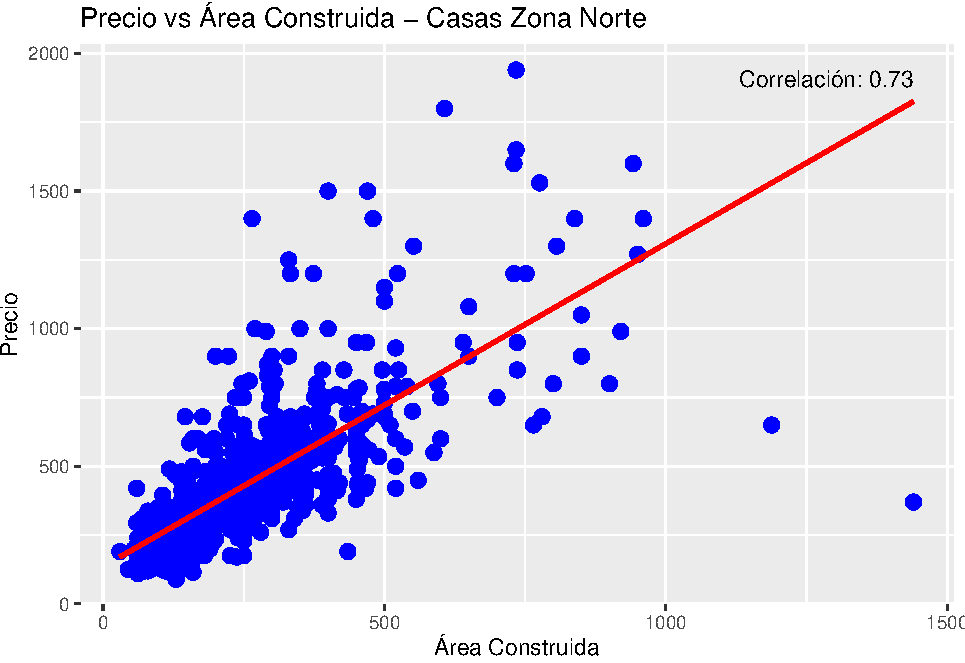
\includegraphics{A2_U2_InformeEjecutivo_files/figure-latex/unnamed-chunk-3-1.pdf}
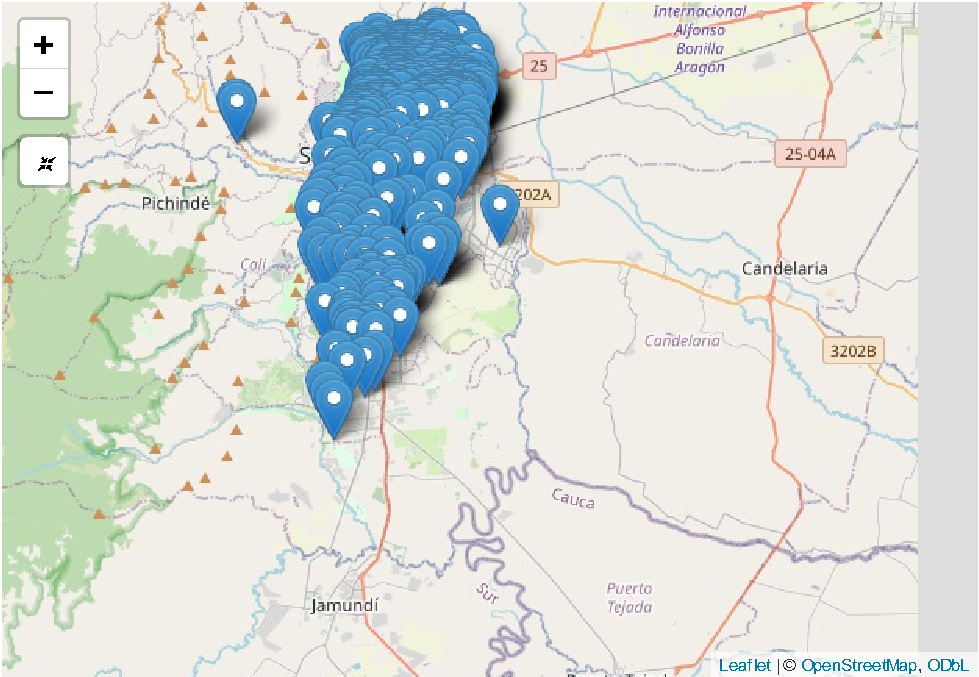
\includegraphics{A2_U2_InformeEjecutivo_files/figure-latex/unnamed-chunk-3-2.pdf}

\begin{verbatim}
## Tabla de frecuencia de tipos de vivienda en la zona norte:
\end{verbatim}

\begin{longtable}[]{@{}lr@{}}
\toprule\noalign{}
Var1 & Freq \\
\midrule\noalign{}
\endhead
\bottomrule\noalign{}
\endlastfoot
Casa & 722 \\
\end{longtable}

\begin{verbatim}
## Tabla de frecuencia de estratos en la zona norte:
\end{verbatim}

\begin{longtable}[]{@{}lr@{}}
\toprule\noalign{}
Var1 & Freq \\
\midrule\noalign{}
\endhead
\bottomrule\noalign{}
\endlastfoot
3 & 235 \\
4 & 161 \\
5 & 271 \\
6 & 55 \\
\end{longtable}

\begin{verbatim}
## Tabla de frecuencia de barrios en la zona norte (ordenada por frecuencia descendente):
\end{verbatim}

\begin{longtable}[]{@{}lr@{}}
\toprule\noalign{}
Var1 & Freq \\
\midrule\noalign{}
\endhead
\bottomrule\noalign{}
\endlastfoot
acopi & 70 \\
brisas de los & 22 \\
alamos & 3 \\
barranquilla & 3 \\
base aérea & 2 \\
alameda del río & 1 \\
atanasio girardot & 1 \\
barrio tranquilo y & 1 \\
berlin & 1 \\
brisas del guabito & 1 \\
\end{longtable}

El gráfico de dispersión evidencia una correlación positiva y robusta
entre el precio de las casas y su área construida en la Zona Norte. Con
un coeficiente de correlación de \textbf{0,73}, se confirma que, en
términos generales, un mayor espacio construido se asocia con un
incremento en el precio de la vivienda.

Por otro lado, la línea de tendencia del gráfico indica que, en
promedio, cada metro cuadrado adicional se traduce en un aumento de
\textbf{1,35 millones} de pesos en el precio, resaltando la influencia
directa del área construida en el valor de la vivienda.

No obstante, la variabilidad observada en torno a esta línea demuestra
que otros factores también tienen un impacto significativo. Aspectos
como la ubicación precisa, la calidad de la construcción, las
características específicas de cada casa y las condiciones generales del
mercado inmobiliario juegan roles determinantes en la fijación del
precio.

Por ello, para realizar una evaluación completa y acertada al momento de
adquirir una vivienda en la Zona Norte, es imprescindible considerar en
conjunto todos estos elementos.

\subsubsection{\texorpdfstring{\textbf{Base 2 Casas Zona
Sur}}{Base 2 Casas Zona Sur}}\label{base-2-casas-zona-sur}

\paragraph{\texorpdfstring{\textbf{Estadísticas Descriptivas de Casas en
la Zona
Sur}}{Estadísticas Descriptivas de Casas en la Zona Sur}}\label{estaduxedsticas-descriptivas-de-casas-en-la-zona-sur}

El análisis descriptivo de las ofertas de casas en la zona sur evidencia
una amplia diversidad en la información recopilada. Con un total de
\textbf{1939} registros, se ha logrado filtrar correctamente el dataset
para incluir únicamente aquellas viviendas ubicadas en esta zona, aunque
se han detectado algunos valores faltantes, lo cual es coherente con la
estructura original del conjunto de datos.

En cuanto a los precios, se observa una gran dispersión: los valores
oscilan entre \textbf{77} y \textbf{1900} unidades monetarias. Tanto la
mediana, que se sitúa en torno a \textbf{480}, como la media, cercana a
\textbf{612.3}, sugieren que la mayoría de las casas se encuentran en
ese rango de precios.

El análisis del área construida también refleja una notable
variabilidad, con dimensiones que van desde \textbf{48} hasta
\textbf{1600} metros cuadrados. Los valores centrales (mediana de
aproximadamente \textbf{247} y media de \textbf{282.3}) indican que la
mayoría de las viviendas presentan áreas construidas en esos rangos.

Además de los precios y el área, otros atributos importantes, como el
número de parqueaderos, baños y habitaciones, muestran una variación
considerable, alcanzando en ocasiones un máximo de 10 unidades. Estos
indicadores son esenciales para comprender las características
específicas y el nivel de comodidad que ofrecen las casas en la zona
sur.

\begin{verbatim}
## Primeros 3 registros de la base de datos filtrada:
\end{verbatim}

\begin{longtable}[]{@{}
  >{\raggedleft\arraybackslash}p{(\columnwidth - 24\tabcolsep) * \real{0.0450}}
  >{\raggedright\arraybackslash}p{(\columnwidth - 24\tabcolsep) * \real{0.0811}}
  >{\raggedright\arraybackslash}p{(\columnwidth - 24\tabcolsep) * \real{0.0450}}
  >{\raggedleft\arraybackslash}p{(\columnwidth - 24\tabcolsep) * \real{0.0721}}
  >{\raggedleft\arraybackslash}p{(\columnwidth - 24\tabcolsep) * \real{0.0721}}
  >{\raggedleft\arraybackslash}p{(\columnwidth - 24\tabcolsep) * \real{0.0901}}
  >{\raggedleft\arraybackslash}p{(\columnwidth - 24\tabcolsep) * \real{0.1171}}
  >{\raggedleft\arraybackslash}p{(\columnwidth - 24\tabcolsep) * \real{0.0631}}
  >{\raggedleft\arraybackslash}p{(\columnwidth - 24\tabcolsep) * \real{0.1171}}
  >{\raggedright\arraybackslash}p{(\columnwidth - 24\tabcolsep) * \real{0.0450}}
  >{\raggedright\arraybackslash}p{(\columnwidth - 24\tabcolsep) * \real{0.0991}}
  >{\raggedleft\arraybackslash}p{(\columnwidth - 24\tabcolsep) * \real{0.0811}}
  >{\raggedleft\arraybackslash}p{(\columnwidth - 24\tabcolsep) * \real{0.0721}}@{}}
\toprule\noalign{}
\begin{minipage}[b]{\linewidth}\raggedleft
id
\end{minipage} & \begin{minipage}[b]{\linewidth}\raggedright
zona
\end{minipage} & \begin{minipage}[b]{\linewidth}\raggedright
piso
\end{minipage} & \begin{minipage}[b]{\linewidth}\raggedleft
estrato
\end{minipage} & \begin{minipage}[b]{\linewidth}\raggedleft
preciom
\end{minipage} & \begin{minipage}[b]{\linewidth}\raggedleft
areaconst
\end{minipage} & \begin{minipage}[b]{\linewidth}\raggedleft
parqueaderos
\end{minipage} & \begin{minipage}[b]{\linewidth}\raggedleft
banios
\end{minipage} & \begin{minipage}[b]{\linewidth}\raggedleft
habitaciones
\end{minipage} & \begin{minipage}[b]{\linewidth}\raggedright
tipo
\end{minipage} & \begin{minipage}[b]{\linewidth}\raggedright
barrio
\end{minipage} & \begin{minipage}[b]{\linewidth}\raggedleft
longitud
\end{minipage} & \begin{minipage}[b]{\linewidth}\raggedleft
latitud
\end{minipage} \\
\midrule\noalign{}
\endhead
\bottomrule\noalign{}
\endlastfoot
5992 & Zona Sur & 02 & 4 & 400 & 280 & 3 & 5 & 3 & Casa & 3 de julio &
-76.540 & 3.435 \\
5157 & Zona Sur & 02 & 3 & 500 & 354 & 1 & 2 & 4 & Casa & alameda &
-76.535 & 3.437 \\
5501 & Zona Sur & 02 & 3 & 175 & 102 & NA & 2 & 4 & Casa & alameda &
-76.537 & 3.435 \\
\end{longtable}

\begin{verbatim}
## Estadísticas descriptivas de las ofertas de casas en la zona sur:
\end{verbatim}

\begin{longtable}[]{@{}
  >{\raggedright\arraybackslash}p{(\columnwidth - 26\tabcolsep) * \real{0.0149}}
  >{\raggedright\arraybackslash}p{(\columnwidth - 26\tabcolsep) * \real{0.0644}}
  >{\raggedright\arraybackslash}p{(\columnwidth - 26\tabcolsep) * \real{0.0842}}
  >{\raggedright\arraybackslash}p{(\columnwidth - 26\tabcolsep) * \real{0.0842}}
  >{\raggedright\arraybackslash}p{(\columnwidth - 26\tabcolsep) * \real{0.0693}}
  >{\raggedright\arraybackslash}p{(\columnwidth - 26\tabcolsep) * \real{0.0743}}
  >{\raggedright\arraybackslash}p{(\columnwidth - 26\tabcolsep) * \real{0.0743}}
  >{\raggedright\arraybackslash}p{(\columnwidth - 26\tabcolsep) * \real{0.0743}}
  >{\raggedright\arraybackslash}p{(\columnwidth - 26\tabcolsep) * \real{0.0743}}
  >{\raggedright\arraybackslash}p{(\columnwidth - 26\tabcolsep) * \real{0.0743}}
  >{\raggedright\arraybackslash}p{(\columnwidth - 26\tabcolsep) * \real{0.0842}}
  >{\raggedright\arraybackslash}p{(\columnwidth - 26\tabcolsep) * \real{0.0842}}
  >{\raggedright\arraybackslash}p{(\columnwidth - 26\tabcolsep) * \real{0.0743}}
  >{\raggedright\arraybackslash}p{(\columnwidth - 26\tabcolsep) * \real{0.0693}}@{}}
\toprule\noalign{}
\begin{minipage}[b]{\linewidth}\raggedright
\end{minipage} & \begin{minipage}[b]{\linewidth}\raggedright
id
\end{minipage} & \begin{minipage}[b]{\linewidth}\raggedright
zona
\end{minipage} & \begin{minipage}[b]{\linewidth}\raggedright
piso
\end{minipage} & \begin{minipage}[b]{\linewidth}\raggedright
estrato
\end{minipage} & \begin{minipage}[b]{\linewidth}\raggedright
preciom
\end{minipage} & \begin{minipage}[b]{\linewidth}\raggedright
areaconst
\end{minipage} & \begin{minipage}[b]{\linewidth}\raggedright
parqueaderos
\end{minipage} & \begin{minipage}[b]{\linewidth}\raggedright
banios
\end{minipage} & \begin{minipage}[b]{\linewidth}\raggedright
habitaciones
\end{minipage} & \begin{minipage}[b]{\linewidth}\raggedright
tipo
\end{minipage} & \begin{minipage}[b]{\linewidth}\raggedright
barrio
\end{minipage} & \begin{minipage}[b]{\linewidth}\raggedright
longitud
\end{minipage} & \begin{minipage}[b]{\linewidth}\raggedright
latitud
\end{minipage} \\
\midrule\noalign{}
\endhead
\bottomrule\noalign{}
\endlastfoot
& Min. : 1 & Length:1939 & Length:1939 & Min. :3.000 & Min. : 77.0 &
Min. : 48.0 & Min. : 1.000 & Min. : 0.000 & Min. : 0.000 & Length:1939 &
Length:1939 & Min. :-76.57 & Min. :3.333 \\
& 1st Qu.:3230 & Class :character & Class :character & 1st Qu.:4.000 &
1st Qu.: 350.0 & 1st Qu.: 163.5 & 1st Qu.: 1.000 & 1st Qu.: 3.000 & 1st
Qu.: 3.000 & Class :character & Class :character & 1st Qu.:-76.54 & 1st
Qu.:3.368 \\
& Median :4941 & Mode :character & Mode :character & Median :5.000 &
Median : 480.0 & Median : 247.0 & Median : 2.000 & Median : 4.000 &
Median : 4.000 & Mode :character & Mode :character & Median :-76.53 &
Median :3.389 \\
& Mean :4691 & NA & NA & Mean :4.842 & Mean : 612.3 & Mean : 282.3 &
Mean : 2.415 & Mean : 4.173 & Mean : 4.514 & NA & NA & Mean :-76.53 &
Mean :3.391 \\
& 3rd Qu.:6264 & NA & NA & 3rd Qu.:6.000 & 3rd Qu.: 780.0 & 3rd Qu.:
350.0 & 3rd Qu.: 3.000 & 3rd Qu.: 5.000 & 3rd Qu.: 5.000 & NA & NA & 3rd
Qu.:-76.53 & 3rd Qu.:3.413 \\
& Max. :8305 & NA & NA & Max. :6.000 & Max. :1900.0 & Max. :1600.0 &
Max. :10.000 & Max. :10.000 & Max. :10.000 & NA & NA & Max. :-76.46 &
Max. :3.485 \\
& NA & NA & NA & NA & NA & NA & NA's :215 & NA & NA & NA & NA & NA &
NA \\
\end{longtable}

\paragraph{\texorpdfstring{\textbf{Gráfico de Dispersión en la Zona
Sur}}{Gráfico de Dispersión en la Zona Sur}}\label{gruxe1fico-de-dispersiuxf3n-en-la-zona-sur}

El gráfico de dispersión correspondiente a la Zona Sur revela un
coeficiente de correlación de \textbf{0.67}, lo que evidencia una
relación positiva y relativamente fuerte entre el precio y el área
construida. Esto indica que, en general, un mayor espacio construido se
asocia con un aumento en el precio de la vivienda.

La línea de tendencia sugiere que, en promedio, cada metro cuadrado
adicional incrementa el precio en aproximadamente \textbf{1.2} millones
de pesos.

No obstante, la amplia dispersión de los puntos alrededor de la línea de
tendencia pone de manifiesto una considerable variabilidad en los
precios, lo que implica la influencia de otros factores adicionales.

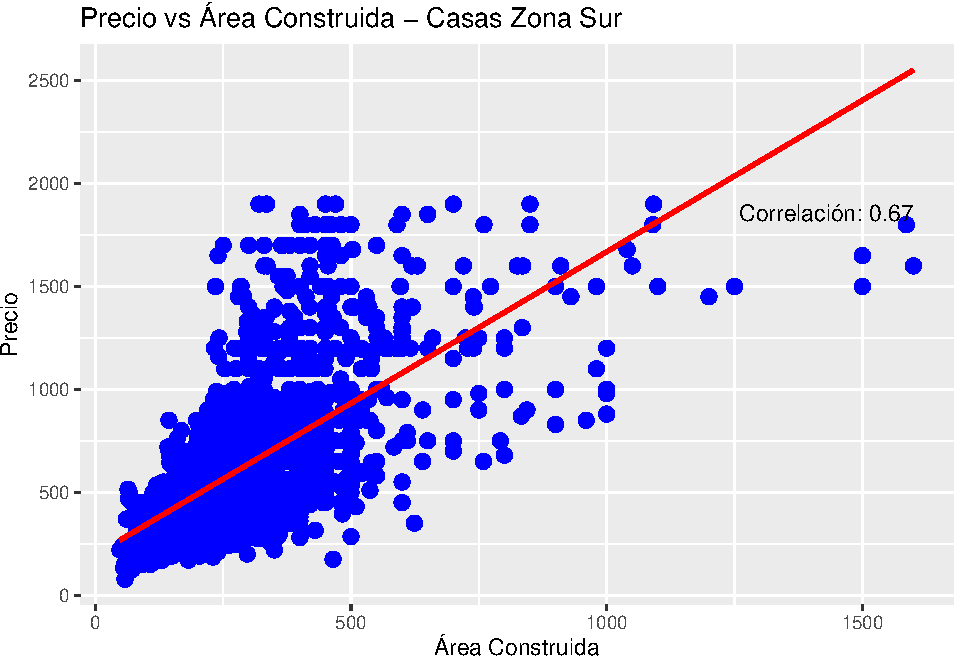
\includegraphics{A2_U2_InformeEjecutivo_files/figure-latex/unnamed-chunk-5-1.pdf}
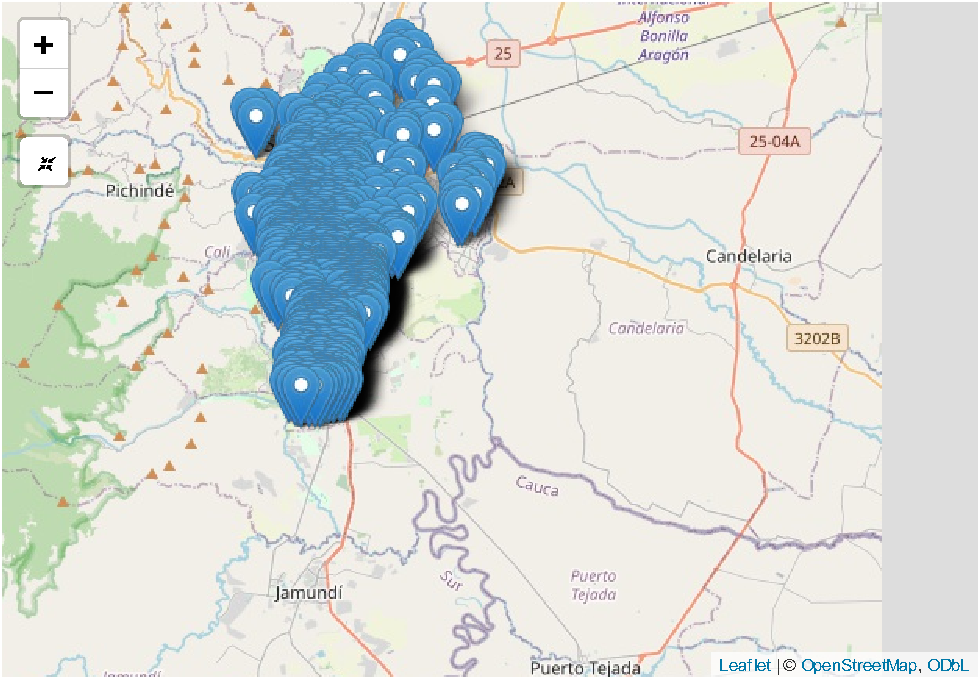
\includegraphics{A2_U2_InformeEjecutivo_files/figure-latex/unnamed-chunk-5-2.pdf}

\begin{verbatim}
## Tabla de frecuencia de tipos de vivienda en la zona sur:
\end{verbatim}

\begin{longtable}[]{@{}lr@{}}
\toprule\noalign{}
Var1 & Freq \\
\midrule\noalign{}
\endhead
\bottomrule\noalign{}
\endlastfoot
Casa & 1939 \\
\end{longtable}

\begin{verbatim}
## Tabla de frecuencia de estratos en la zona sur:
\end{verbatim}

\begin{longtable}[]{@{}lr@{}}
\toprule\noalign{}
Var1 & Freq \\
\midrule\noalign{}
\endhead
\bottomrule\noalign{}
\endlastfoot
3 & 181 \\
4 & 525 \\
5 & 652 \\
6 & 581 \\
\end{longtable}

\begin{verbatim}
## Tabla de frecuencia de barrios en la zona sur (ordenada por frecuencia descendente):
\end{verbatim}

\begin{longtable}[]{@{}lr@{}}
\toprule\noalign{}
Var1 & Freq \\
\midrule\noalign{}
\endhead
\bottomrule\noalign{}
\endlastfoot
alameda & 3 \\
altos de guadalupe & 2 \\
bella suiza alta & 2 \\
3 de julio & 1 \\
alborada & 1 \\
alférez real & 1 \\
alferez real & 1 \\
aranjuez & 1 \\
barrio eucarístico & 1 \\
belalcazar & 1 \\
\end{longtable}

\subsubsection{\texorpdfstring{\textbf{Base 3: Casas en Zona
Oriente}}{Base 3: Casas en Zona Oriente}}\label{base-3-casas-en-zona-oriente}

El análisis descriptivo de las ofertas en la zona oriente evidencia una
distribución de datos similar a la de otras zonas. Este subconjunto,
conformado por \textbf{289} registros, muestra una considerable
variabilidad en los atributos evaluados. Al igual que en otros
conjuntos, se han detectado algunos valores faltantes, lo cual es
consistente con la estructura original del dataset.

En cuanto a los precios, se observa una amplia dispersión: los valores
fluctúan entre \textbf{80} y \textbf{750} unidades monetarias. Tanto la
mediana, situada en \textbf{235}, como la media, en \textbf{244.8},
indican que la mayoría de las propiedades se concentran en este rango de
precios.

El análisis del área construida revela también una diversidad
significativa, con valores que varían desde \textbf{40} hasta
\textbf{1745} metros cuadrados. Los valores centrales ---una mediana de
\textbf{179} y una media de \textbf{213.4} metros cuadrados--- sugieren
que la mayoría de las viviendas presentan áreas construidas en torno a
estos parámetros.

Adicionalmente, otros atributos relevantes, como el \textbf{número de
parqueaderos, baños y habitaciones}, muestran variaciones notables,
alcanzando en algunos casos un máximo de 10 unidades, lo que nos ayuda
para comprender las características y el nivel de equipamiento de las
casas en la zona oriente.

\begin{verbatim}
## Primeros 3 registros de la base de datos filtrada:
\end{verbatim}

\begin{longtable}[]{@{}
  >{\raggedleft\arraybackslash}p{(\columnwidth - 24\tabcolsep) * \real{0.0427}}
  >{\raggedright\arraybackslash}p{(\columnwidth - 24\tabcolsep) * \real{0.1111}}
  >{\raggedright\arraybackslash}p{(\columnwidth - 24\tabcolsep) * \real{0.0427}}
  >{\raggedleft\arraybackslash}p{(\columnwidth - 24\tabcolsep) * \real{0.0684}}
  >{\raggedleft\arraybackslash}p{(\columnwidth - 24\tabcolsep) * \real{0.0684}}
  >{\raggedleft\arraybackslash}p{(\columnwidth - 24\tabcolsep) * \real{0.0855}}
  >{\raggedleft\arraybackslash}p{(\columnwidth - 24\tabcolsep) * \real{0.1111}}
  >{\raggedleft\arraybackslash}p{(\columnwidth - 24\tabcolsep) * \real{0.0598}}
  >{\raggedleft\arraybackslash}p{(\columnwidth - 24\tabcolsep) * \real{0.1111}}
  >{\raggedright\arraybackslash}p{(\columnwidth - 24\tabcolsep) * \real{0.0427}}
  >{\raggedright\arraybackslash}p{(\columnwidth - 24\tabcolsep) * \real{0.1026}}
  >{\raggedleft\arraybackslash}p{(\columnwidth - 24\tabcolsep) * \real{0.0855}}
  >{\raggedleft\arraybackslash}p{(\columnwidth - 24\tabcolsep) * \real{0.0684}}@{}}
\toprule\noalign{}
\begin{minipage}[b]{\linewidth}\raggedleft
id
\end{minipage} & \begin{minipage}[b]{\linewidth}\raggedright
zona
\end{minipage} & \begin{minipage}[b]{\linewidth}\raggedright
piso
\end{minipage} & \begin{minipage}[b]{\linewidth}\raggedleft
estrato
\end{minipage} & \begin{minipage}[b]{\linewidth}\raggedleft
preciom
\end{minipage} & \begin{minipage}[b]{\linewidth}\raggedleft
areaconst
\end{minipage} & \begin{minipage}[b]{\linewidth}\raggedleft
parqueaderos
\end{minipage} & \begin{minipage}[b]{\linewidth}\raggedleft
banios
\end{minipage} & \begin{minipage}[b]{\linewidth}\raggedleft
habitaciones
\end{minipage} & \begin{minipage}[b]{\linewidth}\raggedright
tipo
\end{minipage} & \begin{minipage}[b]{\linewidth}\raggedright
barrio
\end{minipage} & \begin{minipage}[b]{\linewidth}\raggedleft
longitud
\end{minipage} & \begin{minipage}[b]{\linewidth}\raggedleft
latitud
\end{minipage} \\
\midrule\noalign{}
\endhead
\bottomrule\noalign{}
\endlastfoot
1147 & Zona Oriente & NA & 3 & 250 & 70 & 1 & 3 & 6 & Casa & 20 de julio
& -76.51168 & 3.43382 \\
1169 & Zona Oriente & NA & 3 & 320 & 120 & 1 & 2 & 3 & Casa & 20 de
julio & -76.51237 & 3.43369 \\
1350 & Zona Oriente & NA & 3 & 350 & 220 & 2 & 2 & 4 & Casa & 20 de
julio & -76.51537 & 3.43566 \\
\end{longtable}

\begin{verbatim}
## Estadísticas descriptivas de las ofertas de casas en la zona Oriente:
\end{verbatim}

\begin{longtable}[]{@{}
  >{\raggedright\arraybackslash}p{(\columnwidth - 26\tabcolsep) * \real{0.0150}}
  >{\raggedright\arraybackslash}p{(\columnwidth - 26\tabcolsep) * \real{0.0650}}
  >{\raggedright\arraybackslash}p{(\columnwidth - 26\tabcolsep) * \real{0.0850}}
  >{\raggedright\arraybackslash}p{(\columnwidth - 26\tabcolsep) * \real{0.0850}}
  >{\raggedright\arraybackslash}p{(\columnwidth - 26\tabcolsep) * \real{0.0700}}
  >{\raggedright\arraybackslash}p{(\columnwidth - 26\tabcolsep) * \real{0.0700}}
  >{\raggedright\arraybackslash}p{(\columnwidth - 26\tabcolsep) * \real{0.0750}}
  >{\raggedright\arraybackslash}p{(\columnwidth - 26\tabcolsep) * \real{0.0700}}
  >{\raggedright\arraybackslash}p{(\columnwidth - 26\tabcolsep) * \real{0.0750}}
  >{\raggedright\arraybackslash}p{(\columnwidth - 26\tabcolsep) * \real{0.0750}}
  >{\raggedright\arraybackslash}p{(\columnwidth - 26\tabcolsep) * \real{0.0850}}
  >{\raggedright\arraybackslash}p{(\columnwidth - 26\tabcolsep) * \real{0.0850}}
  >{\raggedright\arraybackslash}p{(\columnwidth - 26\tabcolsep) * \real{0.0750}}
  >{\raggedright\arraybackslash}p{(\columnwidth - 26\tabcolsep) * \real{0.0700}}@{}}
\toprule\noalign{}
\begin{minipage}[b]{\linewidth}\raggedright
\end{minipage} & \begin{minipage}[b]{\linewidth}\raggedright
id
\end{minipage} & \begin{minipage}[b]{\linewidth}\raggedright
zona
\end{minipage} & \begin{minipage}[b]{\linewidth}\raggedright
piso
\end{minipage} & \begin{minipage}[b]{\linewidth}\raggedright
estrato
\end{minipage} & \begin{minipage}[b]{\linewidth}\raggedright
preciom
\end{minipage} & \begin{minipage}[b]{\linewidth}\raggedright
areaconst
\end{minipage} & \begin{minipage}[b]{\linewidth}\raggedright
parqueaderos
\end{minipage} & \begin{minipage}[b]{\linewidth}\raggedright
banios
\end{minipage} & \begin{minipage}[b]{\linewidth}\raggedright
habitaciones
\end{minipage} & \begin{minipage}[b]{\linewidth}\raggedright
tipo
\end{minipage} & \begin{minipage}[b]{\linewidth}\raggedright
barrio
\end{minipage} & \begin{minipage}[b]{\linewidth}\raggedright
longitud
\end{minipage} & \begin{minipage}[b]{\linewidth}\raggedright
latitud
\end{minipage} \\
\midrule\noalign{}
\endhead
\bottomrule\noalign{}
\endlastfoot
& Min. : 21 & Length:289 & Length:289 & Min. :3.000 & Min. : 80.0 & Min.
: 40.0 & Min. :1.00 & Min. : 0.000 & Min. : 0.000 & Length:289 &
Length:289 & Min. :-76.56 & Min. :3.389 \\
& 1st Qu.: 424 & Class :character & Class :character & 1st Qu.:3.000 &
1st Qu.:160.0 & 1st Qu.: 122.0 & 1st Qu.:1.00 & 1st Qu.: 2.000 & 1st
Qu.: 3.000 & Class :character & Class :character & 1st Qu.:-76.52 & 1st
Qu.:3.423 \\
& Median : 972 & Mode :character & Mode :character & Median :3.000 &
Median :235.0 & Median : 179.0 & Median :1.00 & Median : 3.000 & Median
: 5.000 & Mode :character & Mode :character & Median :-76.51 & Median
:3.438 \\
& Mean :1277 & NA & NA & Mean :3.028 & Mean :244.8 & Mean : 213.4 & Mean
:1.39 & Mean : 2.965 & Mean : 5.318 & NA & NA & Mean :-76.51 & Mean
:3.434 \\
& 3rd Qu.:1345 & NA & NA & 3rd Qu.:3.000 & 3rd Qu.:310.0 & 3rd Qu.:
252.0 & 3rd Qu.:2.00 & 3rd Qu.: 4.000 & 3rd Qu.: 7.000 & NA & NA & 3rd
Qu.:-76.50 & 3rd Qu.:3.449 \\
& Max. :8271 & NA & NA & Max. :5.000 & Max. :750.0 & Max. :1745.0 & Max.
:6.00 & Max. :10.000 & Max. :10.000 & NA & NA & Max. :-76.47 & Max.
:3.490 \\
& NA & NA & NA & NA & NA & NA & NA's :148 & NA & NA & NA & NA & NA &
NA \\
\end{longtable}

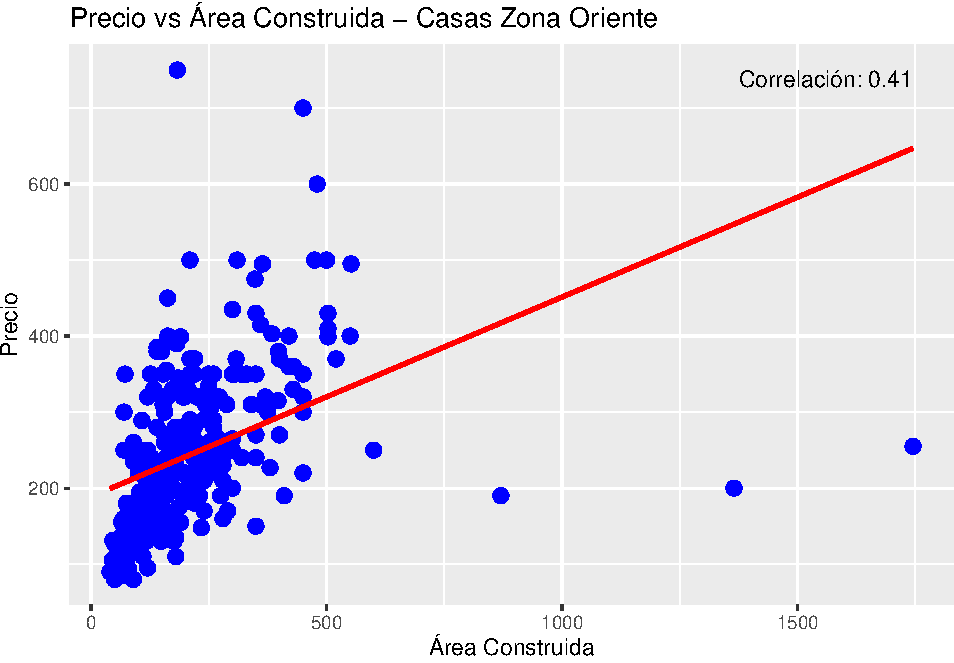
\includegraphics{A2_U2_InformeEjecutivo_files/figure-latex/unnamed-chunk-7-1.pdf}
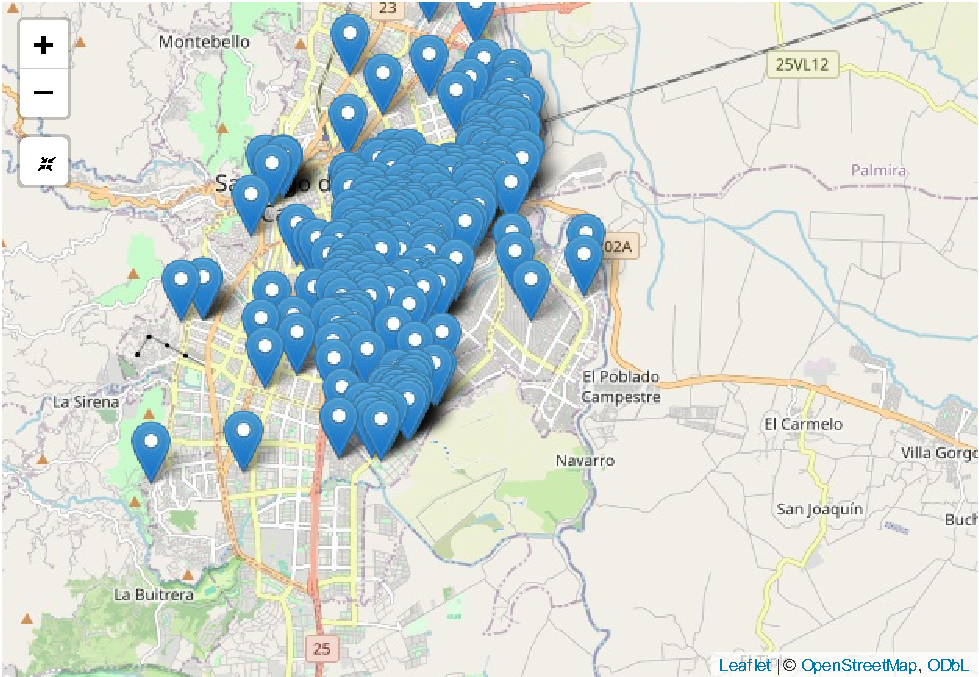
\includegraphics{A2_U2_InformeEjecutivo_files/figure-latex/unnamed-chunk-7-2.pdf}

\begin{verbatim}
## Tabla de frecuencia de tipos de vivienda en la zona oriente:
\end{verbatim}

\begin{longtable}[]{@{}lr@{}}
\toprule\noalign{}
Var1 & Freq \\
\midrule\noalign{}
\endhead
\bottomrule\noalign{}
\endlastfoot
Casa & 289 \\
\end{longtable}

\begin{verbatim}
## Tabla de frecuencia de estratos en la zona oriente:
\end{verbatim}

\begin{longtable}[]{@{}lr@{}}
\toprule\noalign{}
Var1 & Freq \\
\midrule\noalign{}
\endhead
\bottomrule\noalign{}
\endlastfoot
3 & 282 \\
4 & 6 \\
5 & 1 \\
\end{longtable}

\begin{verbatim}
## Tabla de frecuencia de barrios en la zona oriente (ordenada por frecuencia descendente):
\end{verbatim}

\begin{longtable}[]{@{}lr@{}}
\toprule\noalign{}
Var1 & Freq \\
\midrule\noalign{}
\endhead
\bottomrule\noalign{}
\endlastfoot
alfonso lópez & 19 \\
atanasio girardot & 7 \\
20 de julio & 3 \\
antonio nariño & 2 \\
agua blanca & 1 \\
aguablanca & 1 \\
alfonso lopez & 1 \\
alfonso lópez i & 1 \\
arboleda campestre candelaria & 1 \\
autopista sur & 1 \\
\end{longtable}

\paragraph{\texorpdfstring{\textbf{Análisis del Gráfico de Dispersión en
la Zona
Oriente}}{Análisis del Gráfico de Dispersión en la Zona Oriente}}\label{anuxe1lisis-del-gruxe1fico-de-dispersiuxf3n-en-la-zona-oriente}

El análisis del gráfico de dispersión en la Zona Oriente muestra una
correlación positiva moderada entre el \textbf{precio y el área
construida}, con un coeficiente de \textbf{0.41}. Esto indica que,
aunque existe una relación directa en la que a mayor área corresponde un
mayor precio, el impacto del área construida sobre el valor de la
vivienda es menos pronunciado que en las zonas Norte y Sur.

Por otro lado, la línea de tendencia revela que, en promedio, cada metro
cuadrado adicional se traduce en un aumento de aproximadamente
\textbf{0.7 millones} de pesos en el precio. Sin embargo, la notable
dispersión de los puntos en torno a esta línea evidencia una
variabilidad considerable en los precios, lo que sugiere que otros
factores también están influyendo en la determinación del valor.

Esta variabilidad en los precios puede explicarse por la influencia de
otros elementos críticos, tales como la ubicación precisa de la
propiedad, la calidad de la construcción, las características
particulares de cada vivienda y las condiciones específicas del mercado
inmobiliario en la Zona Oriente.

\subsubsection{\texorpdfstring{\textbf{Base 4: Casas en Zona
Oeste}}{Base 4: Casas en Zona Oeste}}\label{base-4-casas-en-zona-oeste}

El análisis descriptivo de las ofertas de casas en la zona oeste muestra
una notable diversidad en la información. Este subconjunto consta de
\textbf{169} registros, lo que evidencia una amplia variabilidad en los
atributos analizados. Al igual que en otras zonas, se han identificado
algunos valores faltantes, lo cual es coherente con la estructura
original del dataset.

En cuanto a los precios, se observa un rango amplio que varía desde
\textbf{135 hasta 1999} unidades monetarias. Tanto la mediana
(aproximadamente \textbf{680}) como la media (alrededor de
\textbf{736.4}) indican que la mayoría de las viviendas se encuentran en
ese rango de precios, reflejando la heterogeneidad del mercado en esta
zona.

El estudio del área construida también resalta una considerable
diversidad, con valores que oscilan entre \textbf{55 y 1200 metros
cuadrados}. Los valores centrales, con una mediana de cerca de
\textbf{300} y una media de aproximadamente \textbf{343.2} metros
cuadrados, sugieren que la mayoría de las casas presentan áreas
construidas en torno a estos parámetros.

\begin{verbatim}
## Primeros 3 registros de la base de datos filtrada:
\end{verbatim}

\begin{longtable}[]{@{}
  >{\raggedleft\arraybackslash}p{(\columnwidth - 24\tabcolsep) * \real{0.0442}}
  >{\raggedright\arraybackslash}p{(\columnwidth - 24\tabcolsep) * \real{0.0973}}
  >{\raggedright\arraybackslash}p{(\columnwidth - 24\tabcolsep) * \real{0.0442}}
  >{\raggedleft\arraybackslash}p{(\columnwidth - 24\tabcolsep) * \real{0.0708}}
  >{\raggedleft\arraybackslash}p{(\columnwidth - 24\tabcolsep) * \real{0.0708}}
  >{\raggedleft\arraybackslash}p{(\columnwidth - 24\tabcolsep) * \real{0.0885}}
  >{\raggedleft\arraybackslash}p{(\columnwidth - 24\tabcolsep) * \real{0.1150}}
  >{\raggedleft\arraybackslash}p{(\columnwidth - 24\tabcolsep) * \real{0.0619}}
  >{\raggedleft\arraybackslash}p{(\columnwidth - 24\tabcolsep) * \real{0.1150}}
  >{\raggedright\arraybackslash}p{(\columnwidth - 24\tabcolsep) * \real{0.0442}}
  >{\raggedright\arraybackslash}p{(\columnwidth - 24\tabcolsep) * \real{0.0885}}
  >{\raggedleft\arraybackslash}p{(\columnwidth - 24\tabcolsep) * \real{0.0885}}
  >{\raggedleft\arraybackslash}p{(\columnwidth - 24\tabcolsep) * \real{0.0708}}@{}}
\toprule\noalign{}
\begin{minipage}[b]{\linewidth}\raggedleft
id
\end{minipage} & \begin{minipage}[b]{\linewidth}\raggedright
zona
\end{minipage} & \begin{minipage}[b]{\linewidth}\raggedright
piso
\end{minipage} & \begin{minipage}[b]{\linewidth}\raggedleft
estrato
\end{minipage} & \begin{minipage}[b]{\linewidth}\raggedleft
preciom
\end{minipage} & \begin{minipage}[b]{\linewidth}\raggedleft
areaconst
\end{minipage} & \begin{minipage}[b]{\linewidth}\raggedleft
parqueaderos
\end{minipage} & \begin{minipage}[b]{\linewidth}\raggedleft
banios
\end{minipage} & \begin{minipage}[b]{\linewidth}\raggedleft
habitaciones
\end{minipage} & \begin{minipage}[b]{\linewidth}\raggedright
tipo
\end{minipage} & \begin{minipage}[b]{\linewidth}\raggedright
barrio
\end{minipage} & \begin{minipage}[b]{\linewidth}\raggedleft
longitud
\end{minipage} & \begin{minipage}[b]{\linewidth}\raggedleft
latitud
\end{minipage} \\
\midrule\noalign{}
\endhead
\bottomrule\noalign{}
\endlastfoot
6928 & Zona Oeste & 03 & 6 & 1850 & 302 & 4 & 4 & 3 & Casa & aguacatal &
-76.54600 & 3.44400 \\
7510 & Zona Oeste & 03 & 6 & 1950 & 400 & 4 & 5 & 3 & Casa & aguacatal &
-76.55000 & 3.45600 \\
7586 & Zona Oeste & 03 & 6 & 870 & 275 & 3 & 5 & 4 & Casa & aguacatal &
-76.55074 & 3.45649 \\
\end{longtable}

\begin{verbatim}
## Estadísticas descriptivas de las ofertas de casas en la zona Oeste:
\end{verbatim}

\begin{longtable}[]{@{}
  >{\raggedright\arraybackslash}p{(\columnwidth - 26\tabcolsep) * \real{0.0151}}
  >{\raggedright\arraybackslash}p{(\columnwidth - 26\tabcolsep) * \real{0.0653}}
  >{\raggedright\arraybackslash}p{(\columnwidth - 26\tabcolsep) * \real{0.0854}}
  >{\raggedright\arraybackslash}p{(\columnwidth - 26\tabcolsep) * \real{0.0854}}
  >{\raggedright\arraybackslash}p{(\columnwidth - 26\tabcolsep) * \real{0.0704}}
  >{\raggedright\arraybackslash}p{(\columnwidth - 26\tabcolsep) * \real{0.0754}}
  >{\raggedright\arraybackslash}p{(\columnwidth - 26\tabcolsep) * \real{0.0754}}
  >{\raggedright\arraybackslash}p{(\columnwidth - 26\tabcolsep) * \real{0.0704}}
  >{\raggedright\arraybackslash}p{(\columnwidth - 26\tabcolsep) * \real{0.0653}}
  >{\raggedright\arraybackslash}p{(\columnwidth - 26\tabcolsep) * \real{0.0754}}
  >{\raggedright\arraybackslash}p{(\columnwidth - 26\tabcolsep) * \real{0.0854}}
  >{\raggedright\arraybackslash}p{(\columnwidth - 26\tabcolsep) * \real{0.0854}}
  >{\raggedright\arraybackslash}p{(\columnwidth - 26\tabcolsep) * \real{0.0754}}
  >{\raggedright\arraybackslash}p{(\columnwidth - 26\tabcolsep) * \real{0.0704}}@{}}
\toprule\noalign{}
\begin{minipage}[b]{\linewidth}\raggedright
\end{minipage} & \begin{minipage}[b]{\linewidth}\raggedright
id
\end{minipage} & \begin{minipage}[b]{\linewidth}\raggedright
zona
\end{minipage} & \begin{minipage}[b]{\linewidth}\raggedright
piso
\end{minipage} & \begin{minipage}[b]{\linewidth}\raggedright
estrato
\end{minipage} & \begin{minipage}[b]{\linewidth}\raggedright
preciom
\end{minipage} & \begin{minipage}[b]{\linewidth}\raggedright
areaconst
\end{minipage} & \begin{minipage}[b]{\linewidth}\raggedright
parqueaderos
\end{minipage} & \begin{minipage}[b]{\linewidth}\raggedright
banios
\end{minipage} & \begin{minipage}[b]{\linewidth}\raggedright
habitaciones
\end{minipage} & \begin{minipage}[b]{\linewidth}\raggedright
tipo
\end{minipage} & \begin{minipage}[b]{\linewidth}\raggedright
barrio
\end{minipage} & \begin{minipage}[b]{\linewidth}\raggedright
longitud
\end{minipage} & \begin{minipage}[b]{\linewidth}\raggedright
latitud
\end{minipage} \\
\midrule\noalign{}
\endhead
\bottomrule\noalign{}
\endlastfoot
& Min. : 2 & Length:169 & Length:169 & Min. :3.000 & Min. : 135.0 & Min.
: 55.0 & Min. :1.000 & Min. :0.00 & Min. : 0.000 & Length:169 &
Length:169 & Min. :-76.57 & Min. :3.398 \\
& 1st Qu.:5836 & Class :character & Class :character & 1st Qu.:4.000 &
1st Qu.: 430.0 & 1st Qu.: 233.0 & 1st Qu.:1.000 & 1st Qu.:3.00 & 1st
Qu.: 4.000 & Class :character & Class :character & 1st Qu.:-76.55 & 1st
Qu.:3.437 \\
& Median :6725 & Mode :character & Mode :character & Median :5.000 &
Median : 680.0 & Median : 300.0 & Median :2.000 & Median :4.00 & Median
: 4.000 & Mode :character & Mode :character & Median :-76.54 & Median
:3.444 \\
& Mean :6235 & NA & NA & Mean :4.899 & Mean : 736.4 & Mean : 343.2 &
Mean :2.311 & Mean :4.26 & Mean : 4.645 & NA & NA & Mean :-76.54 & Mean
:3.443 \\
& 3rd Qu.:7332 & NA & NA & 3rd Qu.:6.000 & 3rd Qu.: 930.0 & 3rd Qu.:
435.0 & 3rd Qu.:3.000 & 3rd Qu.:5.00 & 3rd Qu.: 5.000 & NA & NA & 3rd
Qu.:-76.54 & 3rd Qu.:3.451 \\
& Max. :8311 & NA & NA & Max. :6.000 & Max. :1999.0 & Max. :1200.0 &
Max. :7.000 & Max. :9.00 & Max. :10.000 & NA & NA & Max. :-76.46 & Max.
:3.494 \\
& NA & NA & NA & NA & NA & NA & NA's :37 & NA & NA & NA & NA & NA &
NA \\
\end{longtable}

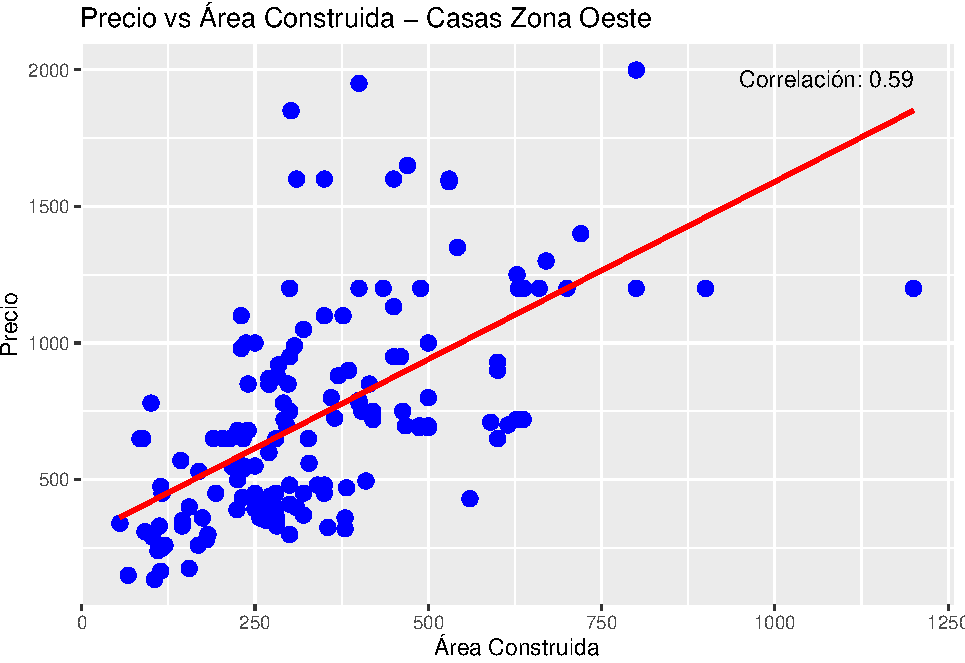
\includegraphics{A2_U2_InformeEjecutivo_files/figure-latex/unnamed-chunk-9-1.pdf}
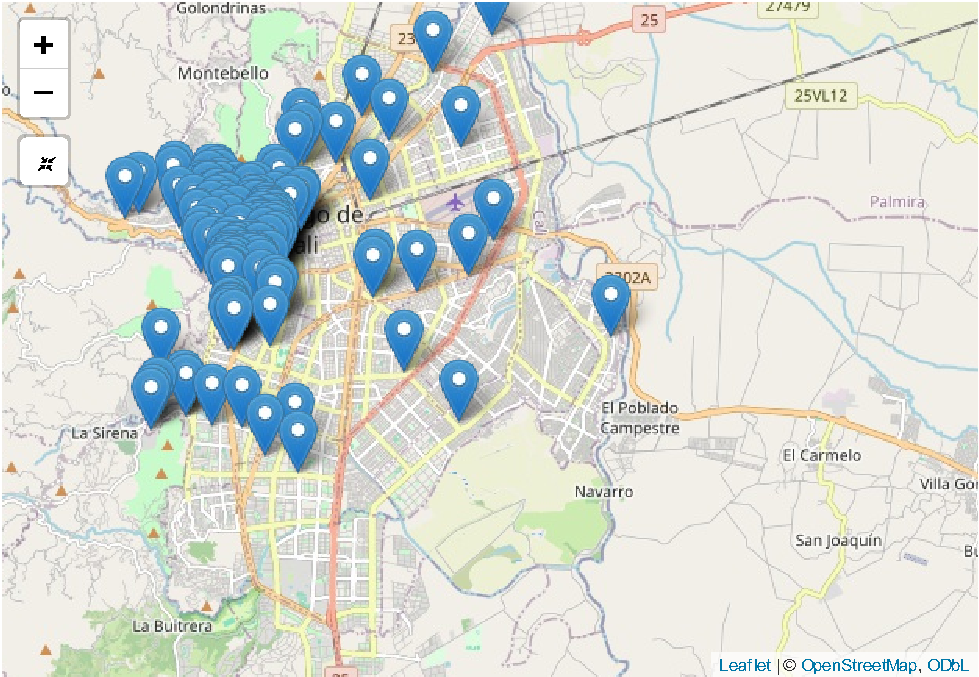
\includegraphics{A2_U2_InformeEjecutivo_files/figure-latex/unnamed-chunk-9-2.pdf}

\begin{verbatim}
## Tabla de frecuencia de tipos de vivienda en la zona Oeste:
\end{verbatim}

\begin{longtable}[]{@{}lr@{}}
\toprule\noalign{}
Var1 & Freq \\
\midrule\noalign{}
\endhead
\bottomrule\noalign{}
\endlastfoot
Casa & 169 \\
\end{longtable}

\begin{verbatim}
## Tabla de frecuencia de estratos en la zona Oeste:
\end{verbatim}

\begin{longtable}[]{@{}lr@{}}
\toprule\noalign{}
Var1 & Freq \\
\midrule\noalign{}
\endhead
\bottomrule\noalign{}
\endlastfoot
3 & 25 \\
4 & 26 \\
5 & 59 \\
6 & 59 \\
\end{longtable}

\begin{verbatim}
## Tabla de frecuencia de barrios en la zona oeste (ordenada por frecuencia descendente):
\end{verbatim}

\begin{longtable}[]{@{}lr@{}}
\toprule\noalign{}
Var1 & Freq \\
\midrule\noalign{}
\endhead
\bottomrule\noalign{}
\endlastfoot
aguacatal & 11 \\
cristales & 10 \\
bella suiza & 7 \\
bellavista & 7 \\
el peñon & 4 \\
altos de guadalupe & 1 \\
bella suiza alta & 1 \\
el nacional & 1 \\
juanamb√∫ & 1 \\
la cascada & 1 \\
\end{longtable}

\paragraph{\texorpdfstring{\textbf{Análisis del Gráfico de Dispersión en
la Zona
Oeste}}{Análisis del Gráfico de Dispersión en la Zona Oeste}}\label{anuxe1lisis-del-gruxe1fico-de-dispersiuxf3n-en-la-zona-oeste}

El gráfico de dispersión para la Zona Oeste evidencia una correlación
moderadamente positiva entre el precio y el área construida, con un
coeficiente de \textbf{0.59}. Esto implica que, si bien existe una
relación directa entre estas variables, el área construida no determina
de manera exclusiva el precio de las viviendas.

Por otro lado, la línea de tendencia indica que, en promedio, cada metro
cuadrado adicional se asocia con un incremento de \textbf{0.95 millones
de pesos} en el precio. No obstante, la marcada dispersión de los puntos
alrededor de esta línea revela una variabilidad considerable en los
precios, lo que sugiere la influencia de otros factores adicionales.

\subsubsection{\texorpdfstring{\textbf{Base 5 Casas Zona
Centro}}{Base 5 Casas Zona Centro}}\label{base-5-casas-zona-centro}

El análisis descriptivo de las ofertas de casas en la zona centro revela
una gran diversidad en los datos, en donde, con un total de 100
registros, se observa una variabilidad significativa en los atributos
evaluados, y, al igual que en otras zonas, se identifican algunos
valores faltantes, lo cual es consistente con la estructura original del
dataset.

Respecto a los precios, se destaca una amplia dispersión: los valores
oscilan entre \textbf{148 y 1100} unidades monetarias. Tanto la mediana,
en torno a \textbf{310}, como la media, aproximadamente \textbf{339.2},
indican que la mayoría de las casas se agrupan en este rango de precios.

Asimismo, el análisis del área construida muestra una notable
diversidad, con dimensiones que varían desde \textbf{74 hasta 750}
\(m^2\). Los valores centrales---una mediana cercana a \textbf{200} y
una media de aproximadamente \textbf{217.8} \(m^2\), sugieren que la
mayoría de las viviendas tienen áreas construidas en esos intervalos.

\begin{verbatim}
## Primeros 3 registros de la base de datos filtrada:
\end{verbatim}

\begin{longtable}[]{@{}
  >{\raggedleft\arraybackslash}p{(\columnwidth - 24\tabcolsep) * \real{0.0446}}
  >{\raggedright\arraybackslash}p{(\columnwidth - 24\tabcolsep) * \real{0.1071}}
  >{\raggedright\arraybackslash}p{(\columnwidth - 24\tabcolsep) * \real{0.0446}}
  >{\raggedleft\arraybackslash}p{(\columnwidth - 24\tabcolsep) * \real{0.0714}}
  >{\raggedleft\arraybackslash}p{(\columnwidth - 24\tabcolsep) * \real{0.0714}}
  >{\raggedleft\arraybackslash}p{(\columnwidth - 24\tabcolsep) * \real{0.0893}}
  >{\raggedleft\arraybackslash}p{(\columnwidth - 24\tabcolsep) * \real{0.1161}}
  >{\raggedleft\arraybackslash}p{(\columnwidth - 24\tabcolsep) * \real{0.0625}}
  >{\raggedleft\arraybackslash}p{(\columnwidth - 24\tabcolsep) * \real{0.1161}}
  >{\raggedright\arraybackslash}p{(\columnwidth - 24\tabcolsep) * \real{0.0446}}
  >{\raggedright\arraybackslash}p{(\columnwidth - 24\tabcolsep) * \real{0.0714}}
  >{\raggedleft\arraybackslash}p{(\columnwidth - 24\tabcolsep) * \real{0.0893}}
  >{\raggedleft\arraybackslash}p{(\columnwidth - 24\tabcolsep) * \real{0.0714}}@{}}
\toprule\noalign{}
\begin{minipage}[b]{\linewidth}\raggedleft
id
\end{minipage} & \begin{minipage}[b]{\linewidth}\raggedright
zona
\end{minipage} & \begin{minipage}[b]{\linewidth}\raggedright
piso
\end{minipage} & \begin{minipage}[b]{\linewidth}\raggedleft
estrato
\end{minipage} & \begin{minipage}[b]{\linewidth}\raggedleft
preciom
\end{minipage} & \begin{minipage}[b]{\linewidth}\raggedleft
areaconst
\end{minipage} & \begin{minipage}[b]{\linewidth}\raggedleft
parqueaderos
\end{minipage} & \begin{minipage}[b]{\linewidth}\raggedleft
banios
\end{minipage} & \begin{minipage}[b]{\linewidth}\raggedleft
habitaciones
\end{minipage} & \begin{minipage}[b]{\linewidth}\raggedright
tipo
\end{minipage} & \begin{minipage}[b]{\linewidth}\raggedright
barrio
\end{minipage} & \begin{minipage}[b]{\linewidth}\raggedleft
longitud
\end{minipage} & \begin{minipage}[b]{\linewidth}\raggedleft
latitud
\end{minipage} \\
\midrule\noalign{}
\endhead
\bottomrule\noalign{}
\endlastfoot
5298 & Zona Centro & 01 & 3 & 650 & 240 & 2 & 4 & 4 & Casa & alameda &
-76.53564 & 3.43521 \\
5107 & Zona Centro & 02 & 4 & 400 & 460 & NA & 5 & 7 & Casa & alameda &
-76.53471 & 3.43627 \\
5117 & Zona Centro & 02 & 3 & 380 & 290 & NA & 4 & 8 & Casa & alameda &
-76.53481 & 3.43712 \\
\end{longtable}

\begin{verbatim}
## Estadísticas descriptivas de las ofertas de casas en la zona Centro:
\end{verbatim}

\begin{longtable}[]{@{}
  >{\raggedright\arraybackslash}p{(\columnwidth - 26\tabcolsep) * \real{0.0153}}
  >{\raggedright\arraybackslash}p{(\columnwidth - 26\tabcolsep) * \real{0.0663}}
  >{\raggedright\arraybackslash}p{(\columnwidth - 26\tabcolsep) * \real{0.0867}}
  >{\raggedright\arraybackslash}p{(\columnwidth - 26\tabcolsep) * \real{0.0867}}
  >{\raggedright\arraybackslash}p{(\columnwidth - 26\tabcolsep) * \real{0.0663}}
  >{\raggedright\arraybackslash}p{(\columnwidth - 26\tabcolsep) * \real{0.0765}}
  >{\raggedright\arraybackslash}p{(\columnwidth - 26\tabcolsep) * \real{0.0714}}
  >{\raggedright\arraybackslash}p{(\columnwidth - 26\tabcolsep) * \real{0.0714}}
  >{\raggedright\arraybackslash}p{(\columnwidth - 26\tabcolsep) * \real{0.0663}}
  >{\raggedright\arraybackslash}p{(\columnwidth - 26\tabcolsep) * \real{0.0714}}
  >{\raggedright\arraybackslash}p{(\columnwidth - 26\tabcolsep) * \real{0.0867}}
  >{\raggedright\arraybackslash}p{(\columnwidth - 26\tabcolsep) * \real{0.0867}}
  >{\raggedright\arraybackslash}p{(\columnwidth - 26\tabcolsep) * \real{0.0765}}
  >{\raggedright\arraybackslash}p{(\columnwidth - 26\tabcolsep) * \real{0.0714}}@{}}
\toprule\noalign{}
\begin{minipage}[b]{\linewidth}\raggedright
\end{minipage} & \begin{minipage}[b]{\linewidth}\raggedright
id
\end{minipage} & \begin{minipage}[b]{\linewidth}\raggedright
zona
\end{minipage} & \begin{minipage}[b]{\linewidth}\raggedright
piso
\end{minipage} & \begin{minipage}[b]{\linewidth}\raggedright
estrato
\end{minipage} & \begin{minipage}[b]{\linewidth}\raggedright
preciom
\end{minipage} & \begin{minipage}[b]{\linewidth}\raggedright
areaconst
\end{minipage} & \begin{minipage}[b]{\linewidth}\raggedright
parqueaderos
\end{minipage} & \begin{minipage}[b]{\linewidth}\raggedright
banios
\end{minipage} & \begin{minipage}[b]{\linewidth}\raggedright
habitaciones
\end{minipage} & \begin{minipage}[b]{\linewidth}\raggedright
tipo
\end{minipage} & \begin{minipage}[b]{\linewidth}\raggedright
barrio
\end{minipage} & \begin{minipage}[b]{\linewidth}\raggedright
longitud
\end{minipage} & \begin{minipage}[b]{\linewidth}\raggedright
latitud
\end{minipage} \\
\midrule\noalign{}
\endhead
\bottomrule\noalign{}
\endlastfoot
& Min. : 572 & Length:100 & Length:100 & Min. :3.00 & Min. : 148.0 &
Min. : 74.0 & Min. :1.000 & Min. :0.00 & Min. : 0.00 & Length:100 &
Length:100 & Min. :-76.54 & Min. :3.398 \\
& 1st Qu.:2976 & Class :character & Class :character & 1st Qu.:3.00 &
1st Qu.: 238.8 & 1st Qu.:146.5 & 1st Qu.:1.000 & 1st Qu.:2.00 & 1st Qu.:
3.00 & Class :character & Class :character & 1st Qu.:-76.53 & 1st
Qu.:3.436 \\
& Median :3739 & Mode :character & Mode :character & Median :3.00 &
Median : 310.0 & Median :200.0 & Median :1.000 & Median :3.00 & Median :
5.00 & Mode :character & Mode :character & Median :-76.53 & Median
:3.439 \\
& Mean :3816 & NA & NA & Mean :3.12 & Mean : 339.2 & Mean :217.8 & Mean
:1.481 & Mean :3.01 & Mean : 5.11 & NA & NA & Mean :-76.53 & Mean
:3.440 \\
& 3rd Qu.:4765 & NA & NA & 3rd Qu.:3.00 & 3rd Qu.: 382.5 & 3rd Qu.:265.5
& 3rd Qu.:1.750 & 3rd Qu.:4.00 & 3rd Qu.: 7.00 & NA & NA & 3rd
Qu.:-76.52 & 3rd Qu.:3.444 \\
& Max. :6662 & NA & NA & Max. :6.00 & Max. :1100.0 & Max. :750.0 & Max.
:6.000 & Max. :9.00 & Max. :10.00 & NA & NA & Max. :-76.50 & Max.
:3.477 \\
& NA & NA & NA & NA & NA & NA & NA's :46 & NA & NA & NA & NA & NA &
NA \\
\end{longtable}

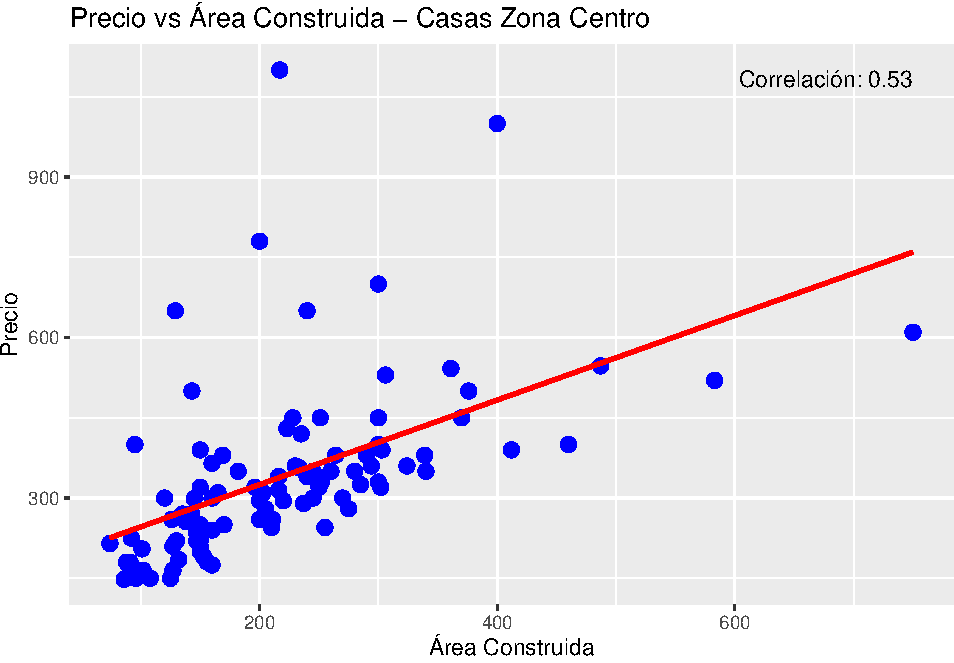
\includegraphics{A2_U2_InformeEjecutivo_files/figure-latex/unnamed-chunk-11-1.pdf}
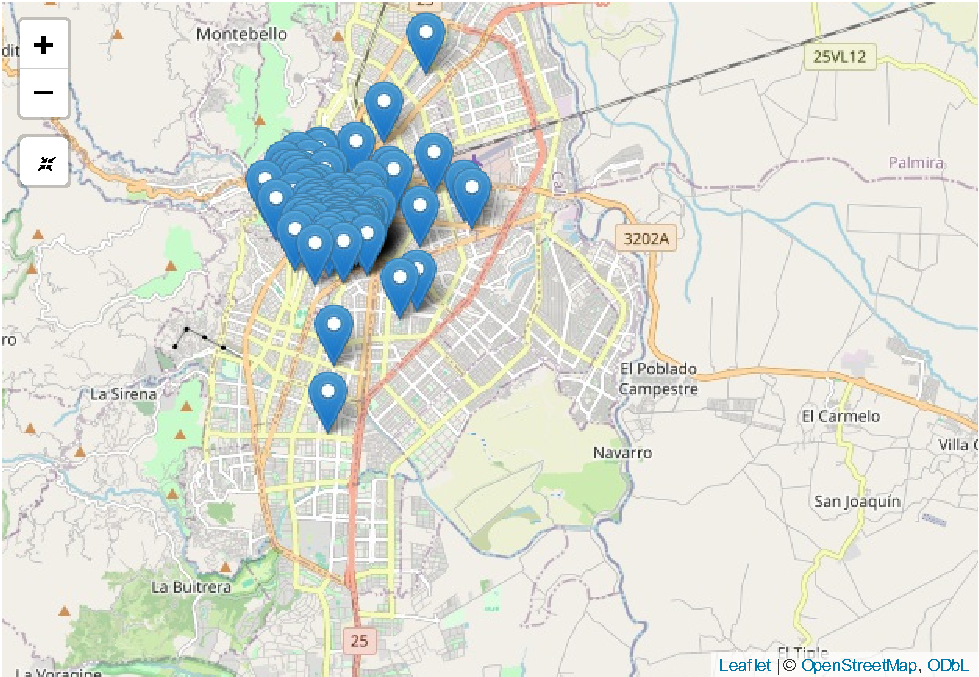
\includegraphics{A2_U2_InformeEjecutivo_files/figure-latex/unnamed-chunk-11-2.pdf}

\begin{verbatim}
## Tabla de frecuencia de tipos de vivienda en la zona Centro:
\end{verbatim}

\begin{longtable}[]{@{}lr@{}}
\toprule\noalign{}
Var1 & Freq \\
\midrule\noalign{}
\endhead
\bottomrule\noalign{}
\endlastfoot
Casa & 100 \\
\end{longtable}

\begin{verbatim}
## Tabla de frecuencia de estratos en la zona Centro:
\end{verbatim}

\begin{longtable}[]{@{}lr@{}}
\toprule\noalign{}
Var1 & Freq \\
\midrule\noalign{}
\endhead
\bottomrule\noalign{}
\endlastfoot
3 & 91 \\
4 & 7 \\
5 & 1 \\
6 & 1 \\
\end{longtable}

\begin{verbatim}
## Tabla de frecuencia de barrios en la zona oriente (ordenada por frecuencia descendente):
\end{verbatim}

\begin{longtable}[]{@{}lr@{}}
\toprule\noalign{}
Var1 & Freq \\
\midrule\noalign{}
\endhead
\bottomrule\noalign{}
\endlastfoot
aranjuez & 14 \\
bretaña & 11 \\
alameda & 9 \\
centro & 3 \\
belalcazar & 2 \\
benjamín herrera & 2 \\
barrio obrero & 1 \\
Belalcazar & 1 \\
colseguros & 1 \\
el troncal & 1 \\
\end{longtable}

\paragraph{\texorpdfstring{\textbf{Gráfico de Dispersión: Zona
Centro}}{Gráfico de Dispersión: Zona Centro}}\label{gruxe1fico-de-dispersiuxf3n-zona-centro}

El gráfico de dispersión correspondiente a la Zona Centro muestra una
correlación moderada y positiva entre el precio y el área construida,
evidenciada por un coeficiente de \textbf{0.53}. Aunque se observa que,
en general, a mayor área corresponde un mayor precio, la influencia del
área construida en el valor de las viviendas es menos determinante que
en otras zonas. La línea de tendencia sugiere que, en promedio, cada
metro cuadrado adicional incrementa el precio en 0.85 millones de pesos.
Sin embargo, la amplia dispersión de los puntos alrededor de esta línea
destaca una variabilidad significativa en los precios, lo que indica la
posible intervención de otros factores en la determinación de los
valores.

\subsubsection{\texorpdfstring{\textbf{Momento de
discusión}}{Momento de discusión}}\label{momento-de-discusiuxf3n}

\paragraph{\texorpdfstring{\textbf{Visualización de la Distribución
Geográfica por
Zona}}{Visualización de la Distribución Geográfica por Zona}}\label{visualizaciuxf3n-de-la-distribuciuxf3n-geogruxe1fica-por-zona}

A continuación, el siguiente mapa ofrece una visión global de cómo se
distribuyen las casas según la zona registrada en el dataset. En este,
se puede observar que ciertos barrios, basándose en sus coordenadas, se
agrupan en la misma zona. Esta coincidencia podría ser atribuida a
errores en el registro de las coordenadas (\textbf{\emph{longitud y
latitud}}) o a equivocaciones en la asignación de la variable
\textbf{\emph{``barrio''}} durante el proceso de captura de datos en el
sistema de información.

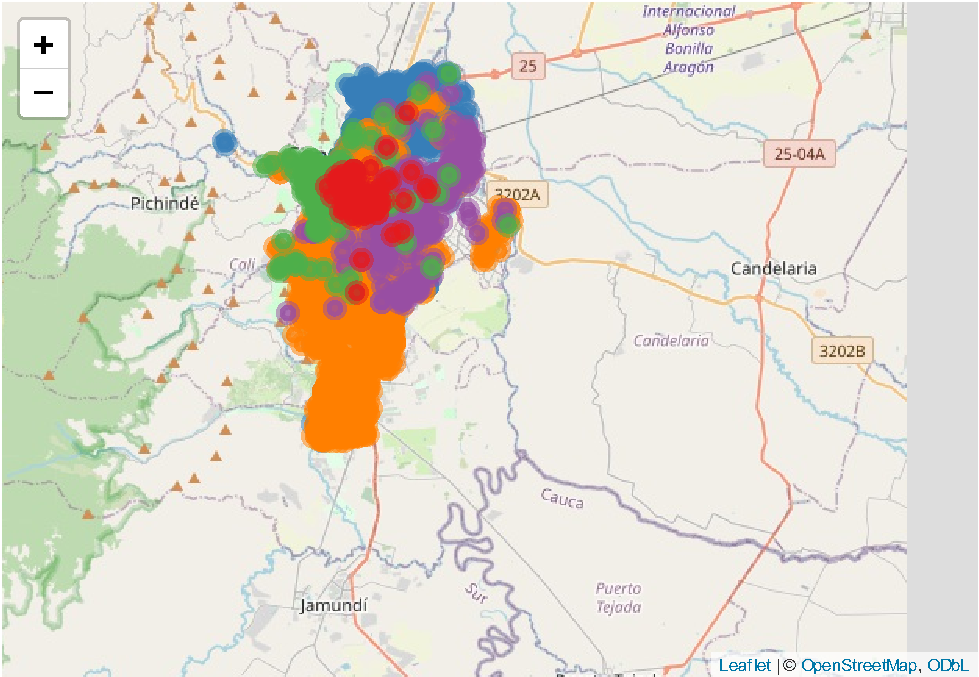
\includegraphics{A2_U2_InformeEjecutivo_files/figure-latex/unnamed-chunk-12-1.pdf}

\subsection{\texorpdfstring{\textbf{2. EDA}}{2. EDA}}\label{eda}

\subsubsection{Correlación del Precio de la Casa con Otras
Variables}\label{correlaciuxf3n-del-precio-de-la-casa-con-otras-variables}

En este apartado se presenta un análisis exploratorio de datos (EDA)
enfocado en estudiar la relación entre el precio de las viviendas
(variable respuesta: \emph{preciom}) y diversas variables predictoras:
área construida (\emph{areaconst}), estrato, número de baños
(\emph{banios}), número de habitaciones y la zona en la que se ubica la
vivienda.

Como resultado del análisis de correlación realizado para el tipo de
vivienda ``Casa'', se han generado dos tipos de gráficos que ayudan a
visualizar estas relaciones:

\begin{itemize}
\item
  \textbf{Gráfico de Dispersión:}\\
  Este gráfico se utiliza para examinar la relación entre dos variables
  cuantitativas. En este contexto, se han trazado gráficos que muestran
  la relación entre el precio y cada una de las siguientes variables:
  área construida, estrato, número de baños y número de habitaciones.
  Cada punto en el gráfico representa una observación del conjunto de
  datos, donde la posición en los ejes \textbf{\emph{x}} e
  \textbf{\emph{y}} indica los valores correspondientes de las dos
  variables analizadas.
\item
  \textbf{Diagrama de Caja y Bigotes (Boxplot):}\\
  Este gráfico permite visualizar la distribución de una variable
  numérica en función de los distintos niveles de una variable
  categórica. En este caso, se ha utilizado para representar la
  distribución de los precios de las viviendas (\textbf{\emph{preciom}})
  en cada una de las zonas. Este tipo de visualización facilita la
  identificación de la mediana, los cuartiles y posibles valores
  atípicos en cada categoría de zona.
\end{itemize}

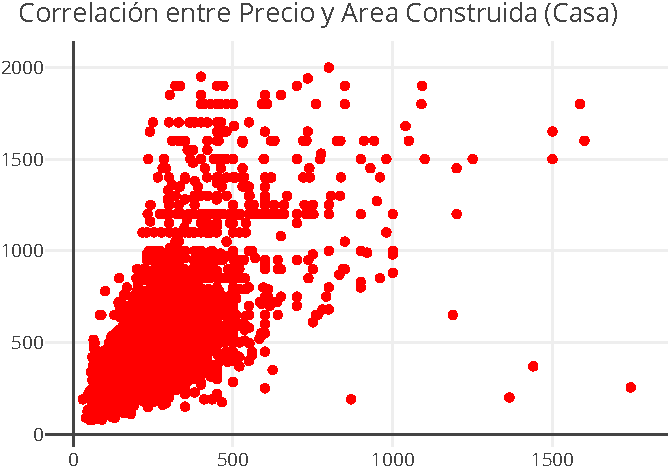
\includegraphics{A2_U2_InformeEjecutivo_files/figure-latex/unnamed-chunk-14-1.pdf}
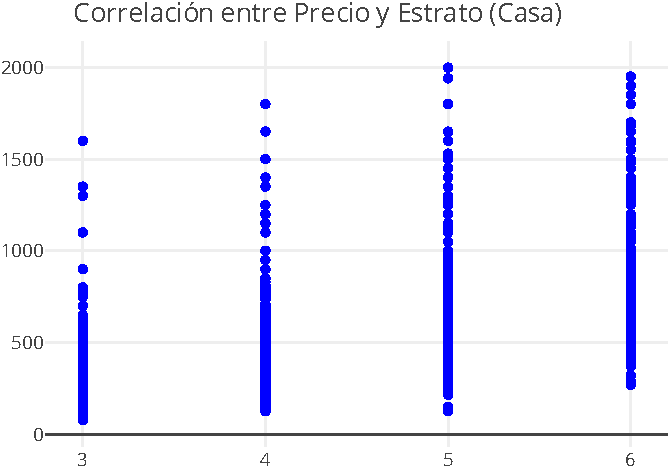
\includegraphics{A2_U2_InformeEjecutivo_files/figure-latex/unnamed-chunk-14-2.pdf}
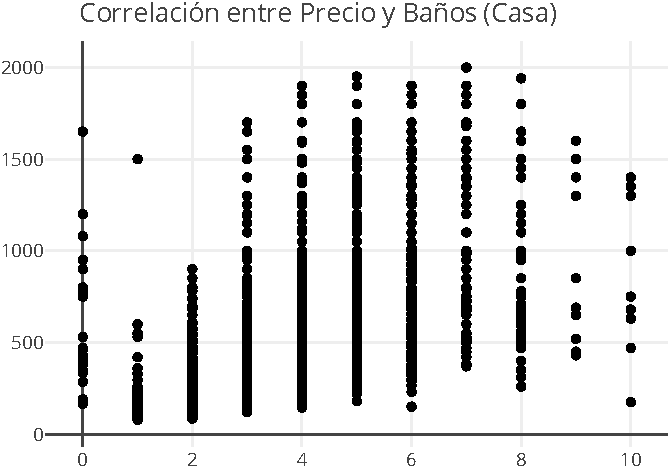
\includegraphics{A2_U2_InformeEjecutivo_files/figure-latex/unnamed-chunk-14-3.pdf}
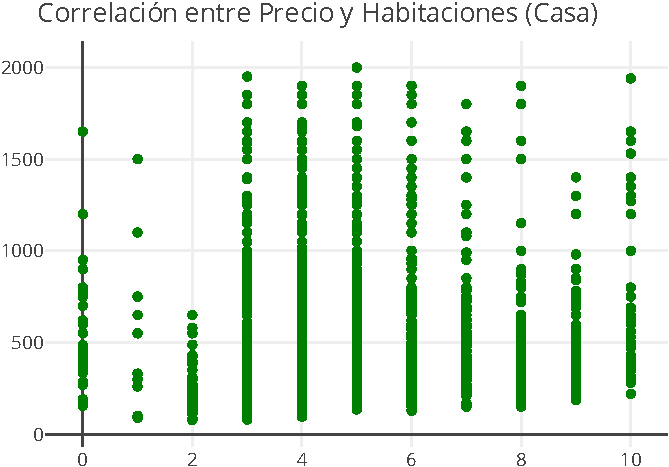
\includegraphics{A2_U2_InformeEjecutivo_files/figure-latex/unnamed-chunk-14-4.pdf}

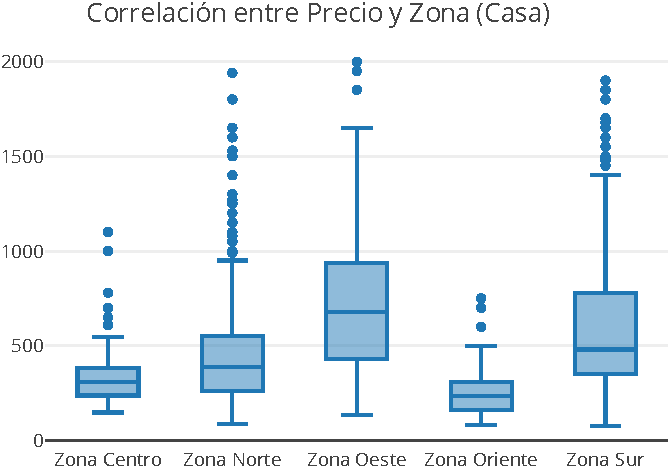
\includegraphics{A2_U2_InformeEjecutivo_files/figure-latex/unnamed-chunk-15-1.pdf}

\begin{verbatim}
##                 preciom areaconst    estrato habitaciones parqueaderos
## preciom      1.00000000 0.6529498  0.6658021   0.09683573           NA
## areaconst    0.65294983 1.0000000  0.3701747   0.28660204           NA
## estrato      0.66580209 0.3701747  1.0000000  -0.11405430           NA
## habitaciones 0.09683573 0.2866020 -0.1140543   1.00000000           NA
## parqueaderos         NA        NA         NA           NA            1
## banios       0.55810021 0.4871721  0.4488832   0.47574058           NA
##                 banios
## preciom      0.5581002
## areaconst    0.4871721
## estrato      0.4488832
## habitaciones 0.4757406
## parqueaderos        NA
## banios       1.0000000
\end{verbatim}

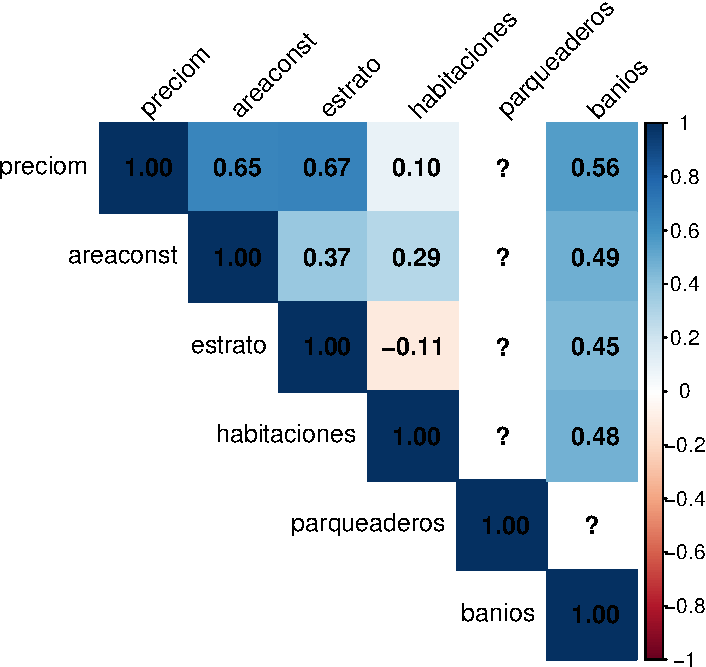
\includegraphics{A2_U2_InformeEjecutivo_files/figure-latex/unnamed-chunk-15-2.pdf}

En base a lo anterior, se puede apreciar que la variable
\textbf{estrato} presenta la correlación más alta con \textbf{preciom}
(\emph{0.6658}), seguida de cerca por \textbf{areaconst} (\emph{0.6529})
y \textbf{banios} (\emph{0.5581}). Estos coeficientes indican que existe
una relación positiva, de moderada a fuerte, entre el precio de la
vivienda y estas características, lo que sugiere que a mayor estrato,
mayor área construida o mayor número de baños, se tiende a observar un
incremento en el precio.

\subsection{\texorpdfstring{\textbf{3. Estimación de un modelo de
regresión lineal
múltiple}}{3. Estimación de un modelo de regresión lineal múltiple}}\label{estimaciuxf3n-de-un-modelo-de-regresiuxf3n-lineal-muxfaltiple}

\begin{verbatim}
## 
## Call:
## lm(formula = preciom ~ areaconst + estrato + habitaciones + parqueaderos + 
##     banios, data = vivienda_casa)
## 
## Residuals:
##      Min       1Q   Median       3Q      Max 
## -1190.80  -114.52   -25.94    74.59   986.16 
## 
## Coefficients:
##                Estimate Std. Error t value Pr(>|t|)    
## (Intercept)  -413.87536   25.58852 -16.174  < 2e-16 ***
## areaconst       0.74227    0.02941  25.235  < 2e-16 ***
## estrato       116.07109    5.26618  22.041  < 2e-16 ***
## habitaciones  -14.74995    3.18137  -4.636 3.73e-06 ***
## parqueaderos   64.29943    3.47719  18.492  < 2e-16 ***
## banios         39.03498    4.05083   9.636  < 2e-16 ***
## ---
## Signif. codes:  0 '***' 0.001 '**' 0.01 '*' 0.05 '.' 0.1 ' ' 1
## 
## Residual standard error: 205.2 on 2480 degrees of freedom
##   (733 observations deleted due to missingness)
## Multiple R-squared:  0.6834, Adjusted R-squared:  0.6828 
## F-statistic:  1071 on 5 and 2480 DF,  p-value: < 2.2e-16
\end{verbatim}

\begin{verbatim}
## [1] 0.6833953
\end{verbatim}

A continuación se presenta la interpretación detallada de los
coeficientes estimados:

\begin{enumerate}
\def\labelenumi{\arabic{enumi}.}
\item
  \textbf{Intercepto}:\\
  El coeficiente del intercepto es \textbf{-413.87536}. Esto indica que,
  en el hipotético caso en que todas las variables predictoras fueran
  iguales a cero, el precio estimado de la vivienda sería de -413.87536
  unidades monetarias. Dado que esta situación no resulta realista en la
  práctica, este valor no posee un significado práctico y se le presta
  poca atención en la interpretación del modelo.
\item
  \textbf{Área Construida}:\\
  Con un coeficiente de \textbf{0.74227}, se interpreta que, manteniendo
  constantes las demás variables, cada unidad adicional en el área
  construida se asocia con un incremento de 0.74227 unidades monetarias
  en el precio de la vivienda.
\item
  \textbf{Estrato}:\\
  El coeficiente para el estrato es \textbf{116.07109}. Esto sugiere
  que, al aumentar en una unidad el estrato (con las demás variables
  fijas), el precio estimado de la vivienda incrementa en 116.07109
  unidades monetarias.
\item
  \textbf{Número de Cuartos (Habitaciones)}:\\
  El coeficiente de \textbf{-14.74995} para el número de cuartos indica
  que, manteniendo constantes las otras variables, cada habitación
  adicional se asocia con una disminución de 14.74995 unidades
  monetarias en el precio estimado. Este resultado sugiere que, en este
  contexto, agregar cuartos podría estar correlacionado con ciertos
  aspectos que reducen el precio, o puede reflejar la presencia de otras
  variables no consideradas.
\item
  \textbf{Número de Parqueaderos}:\\
  Con un coeficiente de \textbf{64.29943}, se deduce que cada
  parqueadero adicional incrementa el precio de la vivienda en 64.29943
  unidades monetarias, al mantener constantes las demás características.
\item
  \textbf{Número de Baños}:\\
  Finalmente, el coeficiente de \textbf{39.03498} para el número de
  baños implica que, controlando por las demás variables, cada baño
  adicional se asocia con un aumento de 39.03498 unidades monetarias en
  el precio de la vivienda.
\end{enumerate}

\subsubsection{\texorpdfstring{\textbf{Gráfico de residuos vs.~valores
ajustados}}{Gráfico de residuos vs.~valores ajustados}}\label{gruxe1fico-de-residuos-vs.-valores-ajustados}

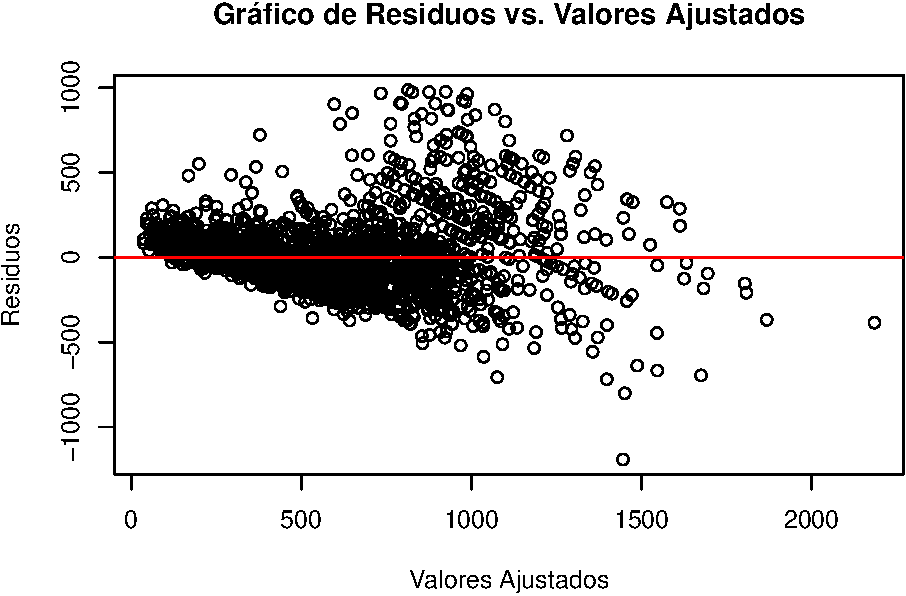
\includegraphics{A2_U2_InformeEjecutivo_files/figure-latex/unnamed-chunk-17-1.pdf}

\subsubsection{\texorpdfstring{\textbf{Gráfico de distribución de los
residuos}}{Gráfico de distribución de los residuos}}\label{gruxe1fico-de-distribuciuxf3n-de-los-residuos}

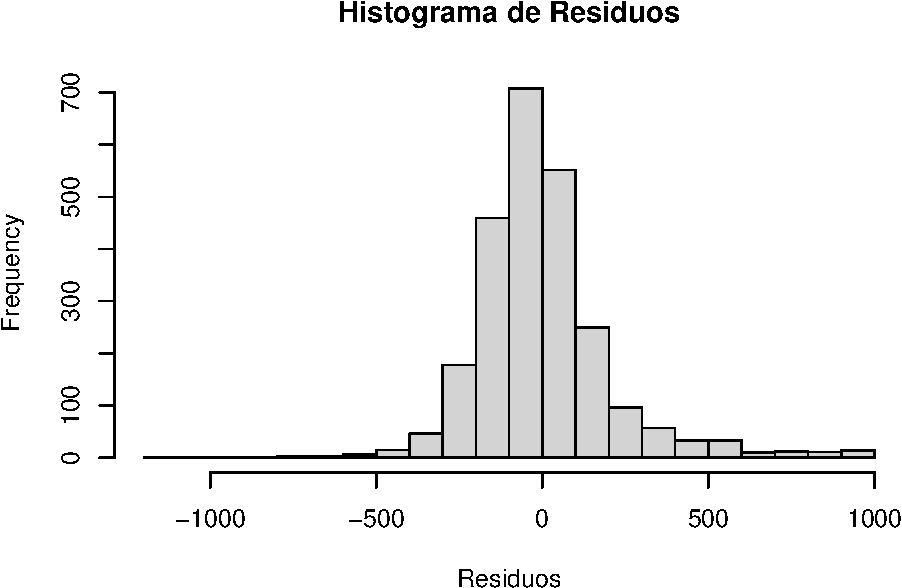
\includegraphics{A2_U2_InformeEjecutivo_files/figure-latex/unnamed-chunk-18-1.pdf}
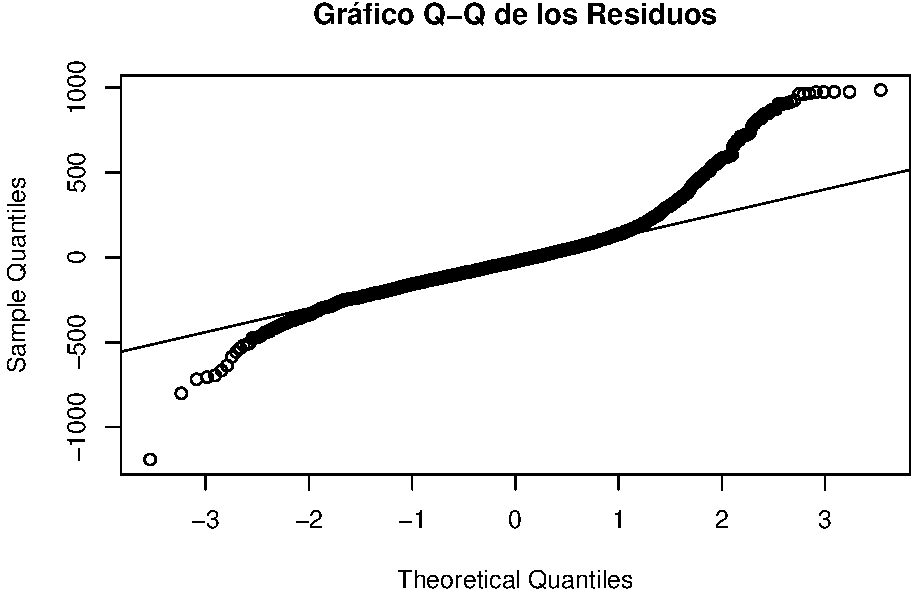
\includegraphics{A2_U2_InformeEjecutivo_files/figure-latex/unnamed-chunk-18-2.pdf}

\subsubsection{\texorpdfstring{\textbf{Gráfico de efectos
parciales}}{Gráfico de efectos parciales}}\label{gruxe1fico-de-efectos-parciales}

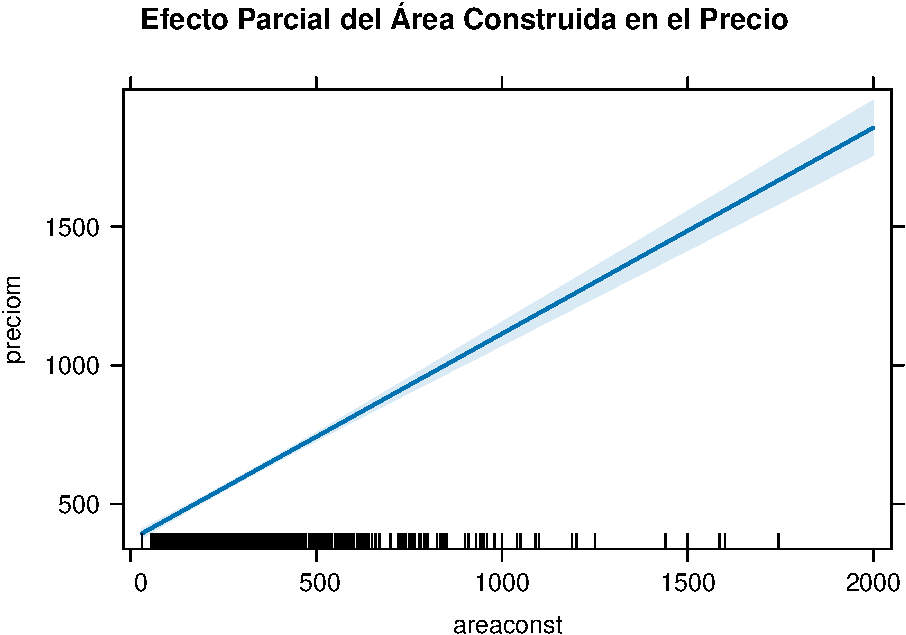
\includegraphics{A2_U2_InformeEjecutivo_files/figure-latex/unnamed-chunk-19-1.pdf}

\subsubsection{\texorpdfstring{\textbf{Gráficos de dispersión con línea
de
regresión}}{Gráficos de dispersión con línea de regresión}}\label{gruxe1ficos-de-dispersiuxf3n-con-luxednea-de-regresiuxf3n}

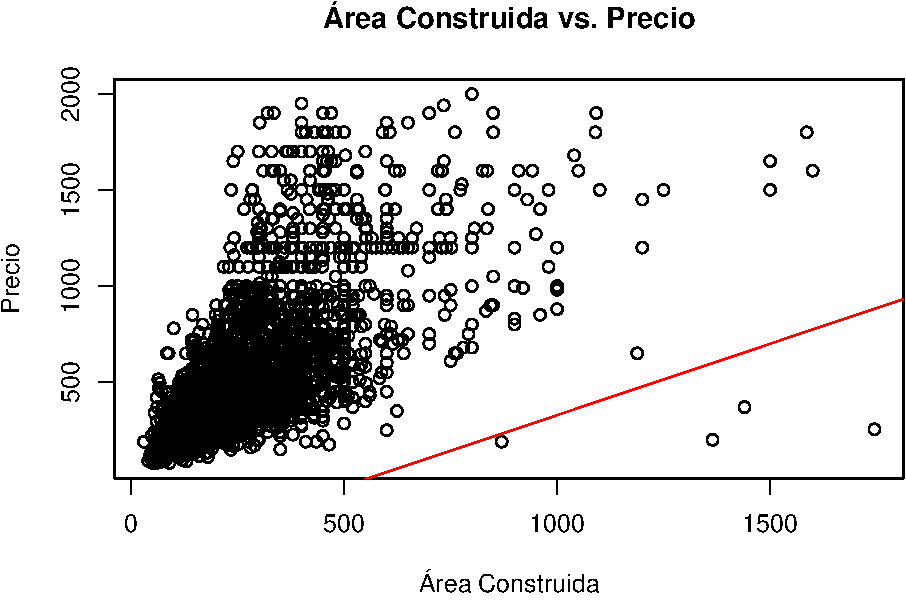
\includegraphics{A2_U2_InformeEjecutivo_files/figure-latex/unnamed-chunk-20-1.pdf}

\subsubsection{\texorpdfstring{\textbf{Interpretación del coeficiente
R²}}{Interpretación del coeficiente R²}}\label{interpretaciuxf3n-del-coeficiente-ruxb2}

El coeficiente de determinación (\textbf{R²}) es de aproximadamente
0.6834, lo que significa que cerca del 68.34\% de la variabilidad en el
precio de la vivienda se puede explicar mediante las variables
independientes incluidas en el modelo. Este valor indica que el ajuste
del modelo a los datos es bueno.

\textbf{Discusión sobre el ajuste del modelo e implicaciones:}

\begin{itemize}
\item
  Un \textbf{R²} relativamente alto sugiere que el modelo de regresión
  lineal múltiple captura una parte significativa de la variabilidad en
  el precio de las propiedades utilizando las variables seleccionadas.
  Sin embargo, siempre existe la posibilidad de mejorar el modelo.
\item
  Se podría considerar la inclusión de variables adicionales relevantes,
  como la ubicación geográfica precisa, la antigüedad de la propiedad o
  características específicas del vecindario, lo que podría aumentar la
  capacidad predictiva del modelo y explicar aún más la variación en los
  precios. Además, explorar transformaciones de las variables existentes
  o utilizar técnicas de modelado más avanzadas puede ayudar a
  perfeccionar la precisión del modelo.
\end{itemize}

\subsection{\texorpdfstring{\textbf{4. Validación de
supuestos}}{4. Validación de supuestos}}\label{validaciuxf3n-de-supuestos}

Esta sección se enfoca en evaluar dos supuestos fundamentales del
análisis de regresión lineal mediante pruebas estadísticas específicas:

\begin{enumerate}
\def\labelenumi{\arabic{enumi}.}
\item
  \textbf{Normalidad de los Residuos:}\\
  Se utiliza la prueba de Shapiro-Wilk para determinar si los residuos
  del modelo se ajustan a una distribución normal. Este supuesto es
  esencial porque el análisis de regresión asume que los errores se
  distribuyen normalmente. Si los residuos se desvían de la normalidad,
  podría ser un indicio de que el modelo no está capturando
  adecuadamente la estructura subyacente de los datos o que existen
  factores adicionales no considerados.
\item
  \textbf{Homocedasticidad de los Residuos:}\\
  La prueba de Breusch-Pagan evalúa si la varianza de los residuos se
  mantiene constante a lo largo de los niveles de las variables
  independientes. La homocedasticidad implica que la dispersión de los
  errores es uniforme en todas las condiciones del modelo. En cambio, si
  se detecta heterocedasticidad, es decir, variaciones en la varianza de
  los residuos, esto podría afectar la precisión de las estimaciones y
  la validez de las pruebas de hipótesis, sugiriendo la necesidad de
  revisar o ajustar el modelo.
\end{enumerate}

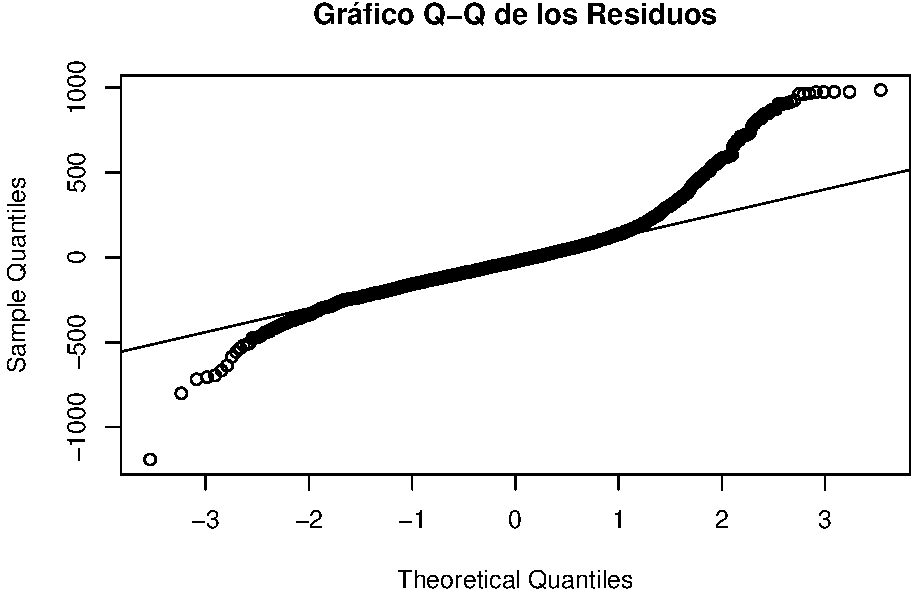
\includegraphics{A2_U2_InformeEjecutivo_files/figure-latex/unnamed-chunk-21-1.pdf}
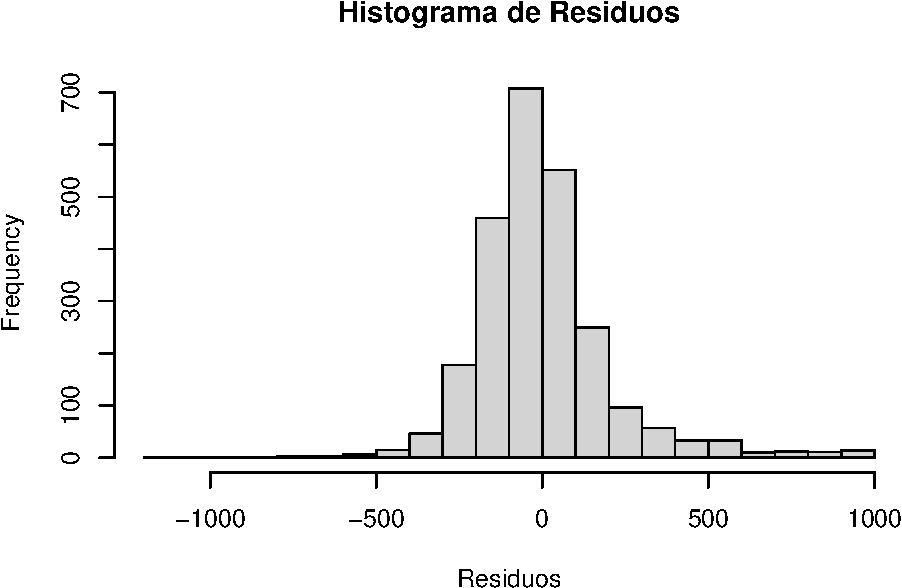
\includegraphics{A2_U2_InformeEjecutivo_files/figure-latex/unnamed-chunk-21-2.pdf}

\begin{verbatim}
## 
##  Shapiro-Wilk normality test
## 
## data:  residuos
## W = 0.89699, p-value < 2.2e-16
\end{verbatim}

\begin{verbatim}
## 
##  studentized Breusch-Pagan test
## 
## data:  modelo_rlm_casa
## BP = 321.2, df = 5, p-value < 2.2e-16
\end{verbatim}

Basado en el análisis de los residuos del modelo de regresión lineal, se
concluye que, aunque los residuos no siguen una distribución normal
perfecta ---como lo indica la prueba de Shapiro-Wilk--- la desviación no
es severa, posiblemente debido al gran tamaño de la muestra. Asimismo,
la prueba de Breusch-Pagan no encontró evidencia de heterocedasticidad,
lo que sugiere que la varianza de los errores se mantiene constante a lo
largo de los niveles de las variables independientes.

\subsection{\texorpdfstring{\textbf{5. Predección del precio de la
vivienda}}{5. Predección del precio de la vivienda}}\label{predecciuxf3n-del-precio-de-la-vivienda}

\begin{verbatim}
##    index precio_predicho
## 1      1        282.1364
## 2      2        296.9818
## 3      3        346.4359
## 5      5        321.1714
## 6      6        336.0168
## 9      9        267.3865
## 10    10        282.2318
## 11    11        331.6859
## 12    12        346.5312
## 13    13        306.4215
## 14    14        321.2668
\end{verbatim}

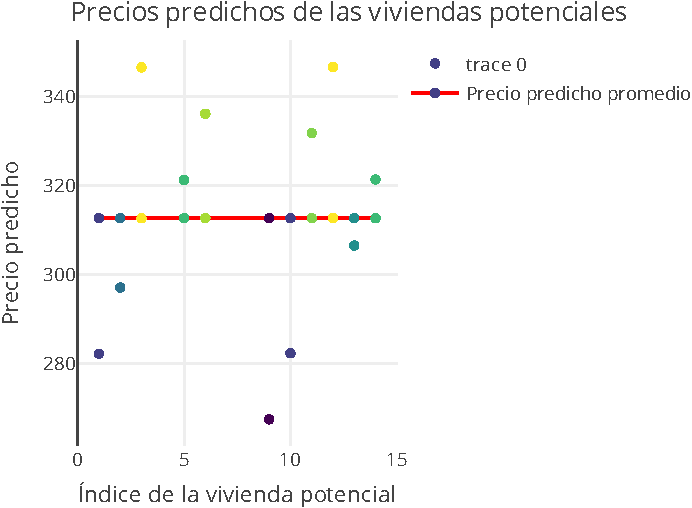
\includegraphics{A2_U2_InformeEjecutivo_files/figure-latex/unnamed-chunk-22-1.pdf}

\subsection{\texorpdfstring{\textbf{6. Ofertas
Potenciales}}{6. Ofertas Potenciales}}\label{ofertas-potenciales}

Los resultados muestran las características de las primeras cinco
viviendas potenciales que cumplen con las condiciones establecidas,
asegurando que su precio estimado no exceda el límite del crédito
preaprobado para la nueva vivienda. A continuación, se describen las
principales características de estas opciones:

\begin{itemize}
\item
  \textbf{Área Construida:}\\
  Las viviendas cuentan con áreas que varían entre 180 y 200 metros
  cuadrados.
\item
  \textbf{Parqueaderos:}\\
  Todas las viviendas disponen de al menos un parqueadero, siendo que
  una de ellas ofrece dos.
\item
  \textbf{Baños:}\\
  La cantidad de baños oscila entre 2 y 3.
\item
  \textbf{Habitaciones:}\\
  Se presentan viviendas con 3 o 4 habitaciones.
\item
  \textbf{Estrato:}\\
  Todas las opciones se ubican en el estrato 4.
\item
  \textbf{Zona:}\\
  Las viviendas están localizadas en la Zona Norte.
\item
  \textbf{Precio Estimado:}\\
  Los precios estimados se sitúan entre 282.1364 y 346.4359 millones de
  pesos.
\end{itemize}

Estos resultados son de gran utilidad para presentar a María las
primeras alternativas de viviendas que cumplen con los criterios
establecidos y se ajustan al presupuesto disponible.

\begin{verbatim}
##   areaconst parqueaderos banios habitaciones estrato       zona precio_estimado
## 1       180            1      2            3       4 Zona Norte        282.1364
## 2       200            1      2            3       4 Zona Norte        296.9818
## 3       180            2      2            3       4 Zona Norte        346.4359
## 5       180            1      3            3       4 Zona Norte        321.1714
## 6       200            1      3            3       4 Zona Norte        336.0168
\end{verbatim}

\subsection{\texorpdfstring{\textbf{7. Escenario de crédito pre-aprobado
para tipo de vivienda
Apartamento}}{7. Escenario de crédito pre-aprobado para tipo de vivienda Apartamento}}\label{escenario-de-cruxe9dito-pre-aprobado-para-tipo-de-vivienda-apartamento}

\subsubsection{\texorpdfstring{\textbf{Segmentación por
zonas}}{Segmentación por zonas}}\label{segmentaciuxf3n-por-zonas}

\paragraph{\texorpdfstring{\textbf{Base 1 Apartamentos Zona
Norte}}{Base 1 Apartamentos Zona Norte}}\label{base-1-apartamentos-zona-norte}

\begin{verbatim}
## Primeros 3 registros de la base de datos filtrada:
\end{verbatim}

\begin{longtable}[]{@{}
  >{\raggedleft\arraybackslash}p{(\columnwidth - 24\tabcolsep) * \real{0.0427}}
  >{\raggedright\arraybackslash}p{(\columnwidth - 24\tabcolsep) * \real{0.0940}}
  >{\raggedright\arraybackslash}p{(\columnwidth - 24\tabcolsep) * \real{0.0427}}
  >{\raggedleft\arraybackslash}p{(\columnwidth - 24\tabcolsep) * \real{0.0684}}
  >{\raggedleft\arraybackslash}p{(\columnwidth - 24\tabcolsep) * \real{0.0684}}
  >{\raggedleft\arraybackslash}p{(\columnwidth - 24\tabcolsep) * \real{0.0855}}
  >{\raggedleft\arraybackslash}p{(\columnwidth - 24\tabcolsep) * \real{0.1111}}
  >{\raggedleft\arraybackslash}p{(\columnwidth - 24\tabcolsep) * \real{0.0598}}
  >{\raggedleft\arraybackslash}p{(\columnwidth - 24\tabcolsep) * \real{0.1111}}
  >{\raggedright\arraybackslash}p{(\columnwidth - 24\tabcolsep) * \real{0.1026}}
  >{\raggedright\arraybackslash}p{(\columnwidth - 24\tabcolsep) * \real{0.0598}}
  >{\raggedleft\arraybackslash}p{(\columnwidth - 24\tabcolsep) * \real{0.0855}}
  >{\raggedleft\arraybackslash}p{(\columnwidth - 24\tabcolsep) * \real{0.0684}}@{}}
\toprule\noalign{}
\begin{minipage}[b]{\linewidth}\raggedleft
id
\end{minipage} & \begin{minipage}[b]{\linewidth}\raggedright
zona
\end{minipage} & \begin{minipage}[b]{\linewidth}\raggedright
piso
\end{minipage} & \begin{minipage}[b]{\linewidth}\raggedleft
estrato
\end{minipage} & \begin{minipage}[b]{\linewidth}\raggedleft
preciom
\end{minipage} & \begin{minipage}[b]{\linewidth}\raggedleft
areaconst
\end{minipage} & \begin{minipage}[b]{\linewidth}\raggedleft
parqueaderos
\end{minipage} & \begin{minipage}[b]{\linewidth}\raggedleft
banios
\end{minipage} & \begin{minipage}[b]{\linewidth}\raggedleft
habitaciones
\end{minipage} & \begin{minipage}[b]{\linewidth}\raggedright
tipo
\end{minipage} & \begin{minipage}[b]{\linewidth}\raggedright
barrio
\end{minipage} & \begin{minipage}[b]{\linewidth}\raggedleft
longitud
\end{minipage} & \begin{minipage}[b]{\linewidth}\raggedleft
latitud
\end{minipage} \\
\midrule\noalign{}
\endhead
\bottomrule\noalign{}
\endlastfoot
1212 & Zona Norte & 01 & 5 & 260 & 90 & 1 & 2 & 3 & Apartamento & acopi
& -76.51350 & 3.45891 \\
1724 & Zona Norte & 01 & 5 & 240 & 87 & 1 & 3 & 3 & Apartamento & acopi
& -76.51700 & 3.36971 \\
2326 & Zona Norte & 01 & 4 & 220 & 52 & 2 & 2 & 3 & Apartamento & acopi
& -76.51974 & 3.42627 \\
\end{longtable}

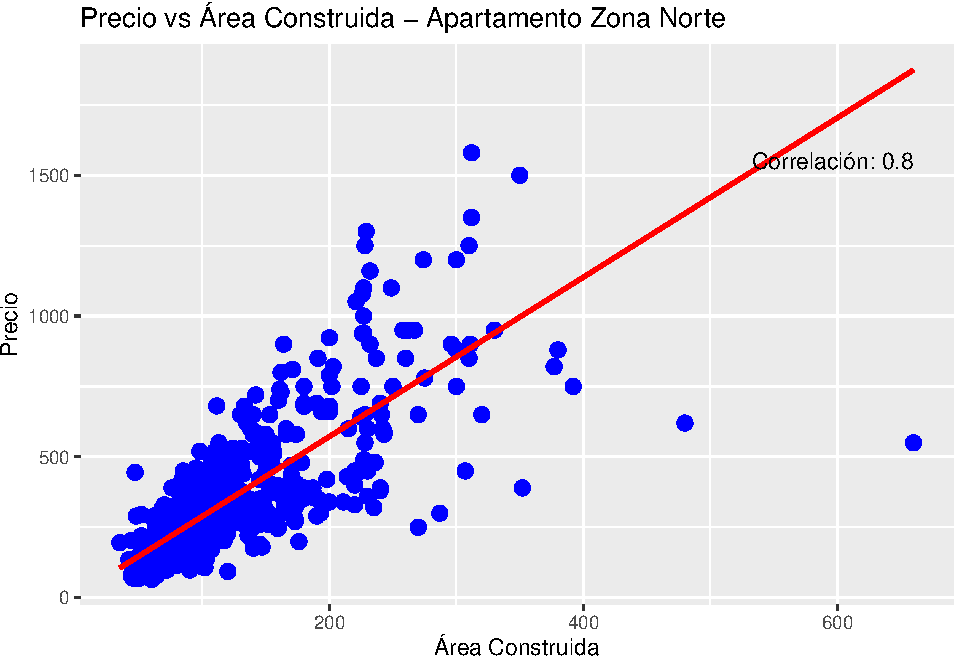
\includegraphics{A2_U2_InformeEjecutivo_files/figure-latex/unnamed-chunk-24-1.pdf}
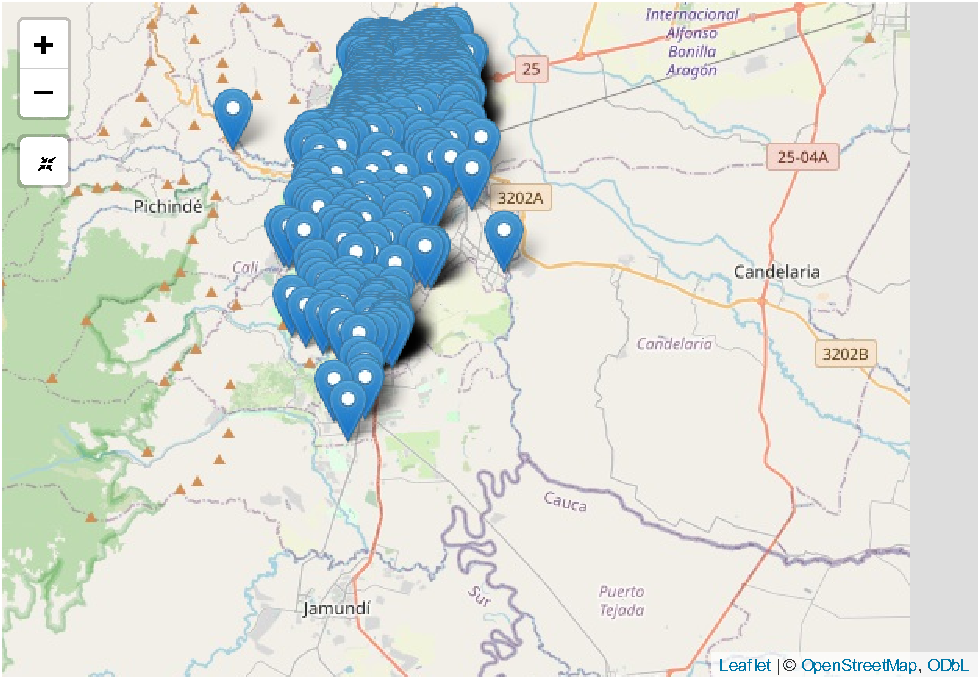
\includegraphics{A2_U2_InformeEjecutivo_files/figure-latex/unnamed-chunk-24-2.pdf}

\paragraph{\texorpdfstring{\textbf{Base 2 Apartamentos Zona
Sur}}{Base 2 Apartamentos Zona Sur}}\label{base-2-apartamentos-zona-sur}

\begin{verbatim}
## Primeros 3 registros de la base de datos filtrada:
\end{verbatim}

\begin{longtable}[]{@{}
  >{\raggedleft\arraybackslash}p{(\columnwidth - 24\tabcolsep) * \real{0.0420}}
  >{\raggedright\arraybackslash}p{(\columnwidth - 24\tabcolsep) * \real{0.0756}}
  >{\raggedright\arraybackslash}p{(\columnwidth - 24\tabcolsep) * \real{0.0420}}
  >{\raggedleft\arraybackslash}p{(\columnwidth - 24\tabcolsep) * \real{0.0672}}
  >{\raggedleft\arraybackslash}p{(\columnwidth - 24\tabcolsep) * \real{0.0672}}
  >{\raggedleft\arraybackslash}p{(\columnwidth - 24\tabcolsep) * \real{0.0840}}
  >{\raggedleft\arraybackslash}p{(\columnwidth - 24\tabcolsep) * \real{0.1092}}
  >{\raggedleft\arraybackslash}p{(\columnwidth - 24\tabcolsep) * \real{0.0588}}
  >{\raggedleft\arraybackslash}p{(\columnwidth - 24\tabcolsep) * \real{0.1092}}
  >{\raggedright\arraybackslash}p{(\columnwidth - 24\tabcolsep) * \real{0.1008}}
  >{\raggedright\arraybackslash}p{(\columnwidth - 24\tabcolsep) * \real{0.0924}}
  >{\raggedleft\arraybackslash}p{(\columnwidth - 24\tabcolsep) * \real{0.0840}}
  >{\raggedleft\arraybackslash}p{(\columnwidth - 24\tabcolsep) * \real{0.0672}}@{}}
\toprule\noalign{}
\begin{minipage}[b]{\linewidth}\raggedleft
id
\end{minipage} & \begin{minipage}[b]{\linewidth}\raggedright
zona
\end{minipage} & \begin{minipage}[b]{\linewidth}\raggedright
piso
\end{minipage} & \begin{minipage}[b]{\linewidth}\raggedleft
estrato
\end{minipage} & \begin{minipage}[b]{\linewidth}\raggedleft
preciom
\end{minipage} & \begin{minipage}[b]{\linewidth}\raggedleft
areaconst
\end{minipage} & \begin{minipage}[b]{\linewidth}\raggedleft
parqueaderos
\end{minipage} & \begin{minipage}[b]{\linewidth}\raggedleft
banios
\end{minipage} & \begin{minipage}[b]{\linewidth}\raggedleft
habitaciones
\end{minipage} & \begin{minipage}[b]{\linewidth}\raggedright
tipo
\end{minipage} & \begin{minipage}[b]{\linewidth}\raggedright
barrio
\end{minipage} & \begin{minipage}[b]{\linewidth}\raggedleft
longitud
\end{minipage} & \begin{minipage}[b]{\linewidth}\raggedleft
latitud
\end{minipage} \\
\midrule\noalign{}
\endhead
\bottomrule\noalign{}
\endlastfoot
5098 & Zona Sur & 05 & 4 & 290 & 96 & 1 & 2 & 3 & Apartamento & acopi &
-76.53464 & 3.44987 \\
698 & Zona Sur & 02 & 3 & 78 & 40 & 1 & 1 & 2 & Apartamento & aguablanca
& -76.50100 & 3.40000 \\
8199 & Zona Sur & NA & 6 & 875 & 194 & 2 & 5 & 3 & Apartamento &
aguacatal & -76.55700 & 3.45900 \\
\end{longtable}

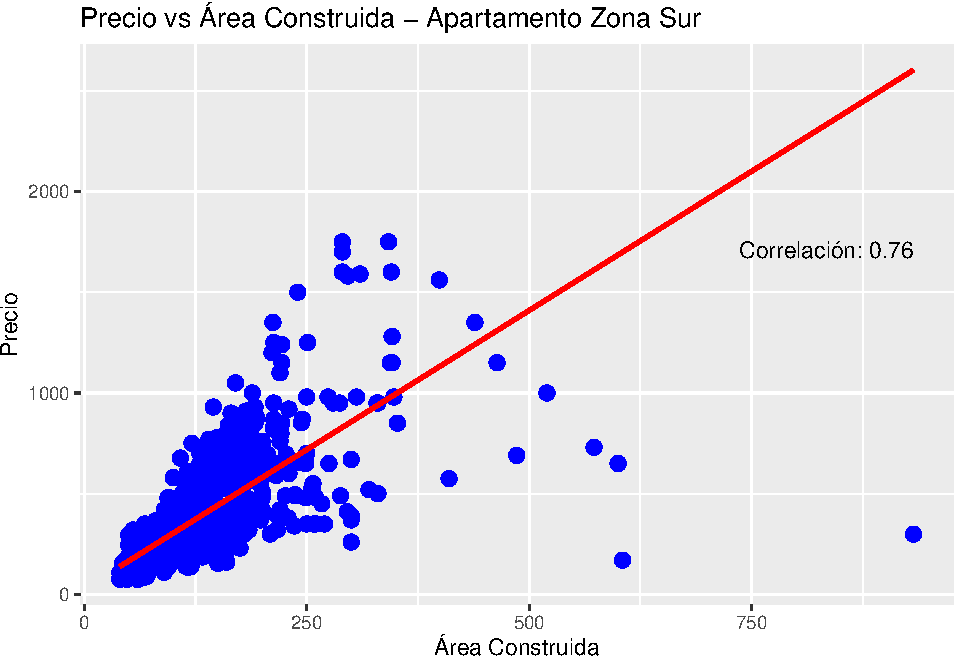
\includegraphics{A2_U2_InformeEjecutivo_files/figure-latex/unnamed-chunk-25-1.pdf}
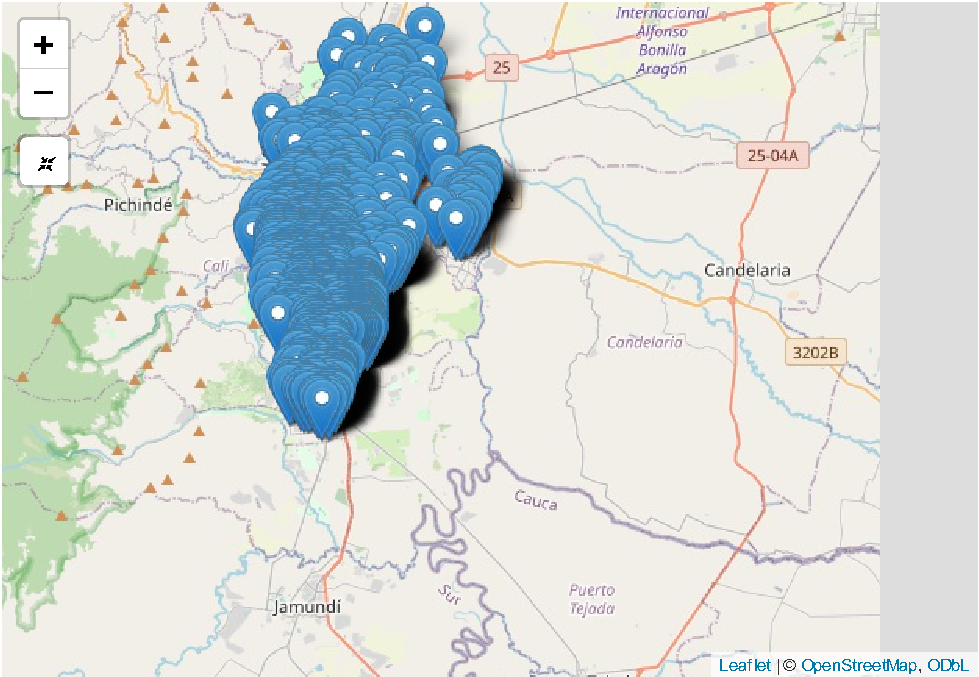
\includegraphics{A2_U2_InformeEjecutivo_files/figure-latex/unnamed-chunk-25-2.pdf}

\paragraph{\texorpdfstring{\textbf{Base 2 Apartamentos Zona
Oeste}}{Base 2 Apartamentos Zona Oeste}}\label{base-2-apartamentos-zona-oeste}

\begin{verbatim}
## Primeros 3 registros de la base de datos filtrada:
\end{verbatim}

\begin{longtable}[]{@{}
  >{\raggedleft\arraybackslash}p{(\columnwidth - 24\tabcolsep) * \real{0.0417}}
  >{\raggedright\arraybackslash}p{(\columnwidth - 24\tabcolsep) * \real{0.0917}}
  >{\raggedright\arraybackslash}p{(\columnwidth - 24\tabcolsep) * \real{0.0417}}
  >{\raggedleft\arraybackslash}p{(\columnwidth - 24\tabcolsep) * \real{0.0667}}
  >{\raggedleft\arraybackslash}p{(\columnwidth - 24\tabcolsep) * \real{0.0667}}
  >{\raggedleft\arraybackslash}p{(\columnwidth - 24\tabcolsep) * \real{0.0833}}
  >{\raggedleft\arraybackslash}p{(\columnwidth - 24\tabcolsep) * \real{0.1083}}
  >{\raggedleft\arraybackslash}p{(\columnwidth - 24\tabcolsep) * \real{0.0583}}
  >{\raggedleft\arraybackslash}p{(\columnwidth - 24\tabcolsep) * \real{0.1083}}
  >{\raggedright\arraybackslash}p{(\columnwidth - 24\tabcolsep) * \real{0.1000}}
  >{\raggedright\arraybackslash}p{(\columnwidth - 24\tabcolsep) * \real{0.0833}}
  >{\raggedleft\arraybackslash}p{(\columnwidth - 24\tabcolsep) * \real{0.0833}}
  >{\raggedleft\arraybackslash}p{(\columnwidth - 24\tabcolsep) * \real{0.0667}}@{}}
\toprule\noalign{}
\begin{minipage}[b]{\linewidth}\raggedleft
id
\end{minipage} & \begin{minipage}[b]{\linewidth}\raggedright
zona
\end{minipage} & \begin{minipage}[b]{\linewidth}\raggedright
piso
\end{minipage} & \begin{minipage}[b]{\linewidth}\raggedleft
estrato
\end{minipage} & \begin{minipage}[b]{\linewidth}\raggedleft
preciom
\end{minipage} & \begin{minipage}[b]{\linewidth}\raggedleft
areaconst
\end{minipage} & \begin{minipage}[b]{\linewidth}\raggedleft
parqueaderos
\end{minipage} & \begin{minipage}[b]{\linewidth}\raggedleft
banios
\end{minipage} & \begin{minipage}[b]{\linewidth}\raggedleft
habitaciones
\end{minipage} & \begin{minipage}[b]{\linewidth}\raggedright
tipo
\end{minipage} & \begin{minipage}[b]{\linewidth}\raggedright
barrio
\end{minipage} & \begin{minipage}[b]{\linewidth}\raggedleft
longitud
\end{minipage} & \begin{minipage}[b]{\linewidth}\raggedleft
latitud
\end{minipage} \\
\midrule\noalign{}
\endhead
\bottomrule\noalign{}
\endlastfoot
6999 & Zona Oeste & 01 & 6 & 870 & 200 & 2 & 5 & 3 & Apartamento &
aguacatal & -76.54666 & 3.44624 \\
8037 & Zona Oeste & 01 & 4 & 130 & 50 & NA & 1 & 3 & Apartamento &
aguacatal & -76.55409 & 3.44338 \\
8055 & Zona Oeste & 01 & 4 & 165 & 61 & 1 & 2 & 3 & Apartamento &
aguacatal & -76.55447 & 3.45783 \\
\end{longtable}

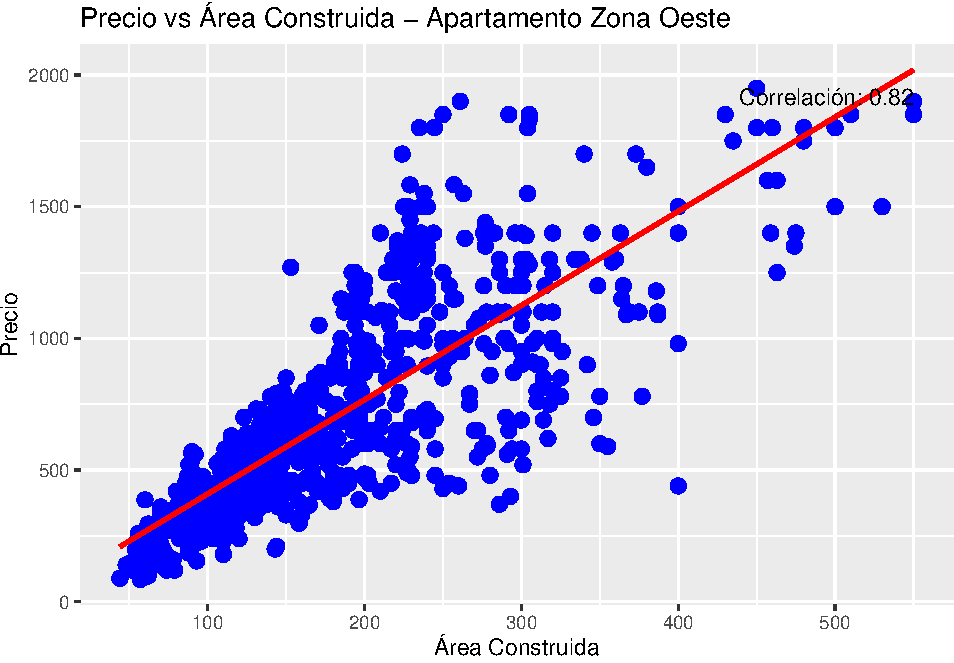
\includegraphics{A2_U2_InformeEjecutivo_files/figure-latex/unnamed-chunk-26-1.pdf}
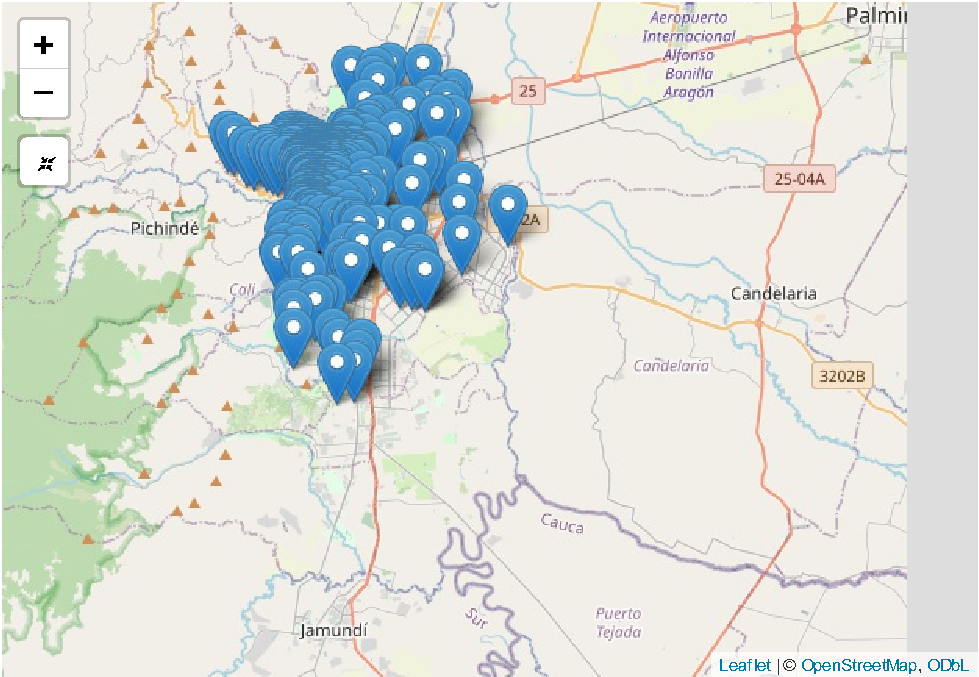
\includegraphics{A2_U2_InformeEjecutivo_files/figure-latex/unnamed-chunk-26-2.pdf}

\paragraph{\texorpdfstring{\textbf{Base 2 Apartamentos Zona
Oriente}}{Base 2 Apartamentos Zona Oriente}}\label{base-2-apartamentos-zona-oriente}

\begin{verbatim}
## Primeros 3 registros de la base de datos filtrada:
\end{verbatim}

\begin{longtable}[]{@{}
  >{\raggedleft\arraybackslash}p{(\columnwidth - 24\tabcolsep) * \real{0.0310}}
  >{\raggedright\arraybackslash}p{(\columnwidth - 24\tabcolsep) * \real{0.1008}}
  >{\raggedright\arraybackslash}p{(\columnwidth - 24\tabcolsep) * \real{0.0388}}
  >{\raggedleft\arraybackslash}p{(\columnwidth - 24\tabcolsep) * \real{0.0620}}
  >{\raggedleft\arraybackslash}p{(\columnwidth - 24\tabcolsep) * \real{0.0620}}
  >{\raggedleft\arraybackslash}p{(\columnwidth - 24\tabcolsep) * \real{0.0775}}
  >{\raggedleft\arraybackslash}p{(\columnwidth - 24\tabcolsep) * \real{0.1008}}
  >{\raggedleft\arraybackslash}p{(\columnwidth - 24\tabcolsep) * \real{0.0543}}
  >{\raggedleft\arraybackslash}p{(\columnwidth - 24\tabcolsep) * \real{0.1008}}
  >{\raggedright\arraybackslash}p{(\columnwidth - 24\tabcolsep) * \real{0.0930}}
  >{\raggedright\arraybackslash}p{(\columnwidth - 24\tabcolsep) * \real{0.1395}}
  >{\raggedleft\arraybackslash}p{(\columnwidth - 24\tabcolsep) * \real{0.0775}}
  >{\raggedleft\arraybackslash}p{(\columnwidth - 24\tabcolsep) * \real{0.0620}}@{}}
\toprule\noalign{}
\begin{minipage}[b]{\linewidth}\raggedleft
id
\end{minipage} & \begin{minipage}[b]{\linewidth}\raggedright
zona
\end{minipage} & \begin{minipage}[b]{\linewidth}\raggedright
piso
\end{minipage} & \begin{minipage}[b]{\linewidth}\raggedleft
estrato
\end{minipage} & \begin{minipage}[b]{\linewidth}\raggedleft
preciom
\end{minipage} & \begin{minipage}[b]{\linewidth}\raggedleft
areaconst
\end{minipage} & \begin{minipage}[b]{\linewidth}\raggedleft
parqueaderos
\end{minipage} & \begin{minipage}[b]{\linewidth}\raggedleft
banios
\end{minipage} & \begin{minipage}[b]{\linewidth}\raggedleft
habitaciones
\end{minipage} & \begin{minipage}[b]{\linewidth}\raggedright
tipo
\end{minipage} & \begin{minipage}[b]{\linewidth}\raggedright
barrio
\end{minipage} & \begin{minipage}[b]{\linewidth}\raggedleft
longitud
\end{minipage} & \begin{minipage}[b]{\linewidth}\raggedleft
latitud
\end{minipage} \\
\midrule\noalign{}
\endhead
\bottomrule\noalign{}
\endlastfoot
82 & Zona Oriente & 01 & 3 & 115 & 111 & 1 & 2 & 4 & Apartamento &
alfonso lópez & -76.48141 & 3.45379 \\
78 & Zona Oriente & 02 & 3 & 58 & 50 & 1 & 1 & 2 & Apartamento & alfonso
lópez & -76.47978 & 3.45131 \\
999 & Zona Oriente & 02 & 3 & 135 & 120 & NA & 2 & 4 & Apartamento &
atanasio girardot & -76.50737 & 3.44454 \\
\end{longtable}

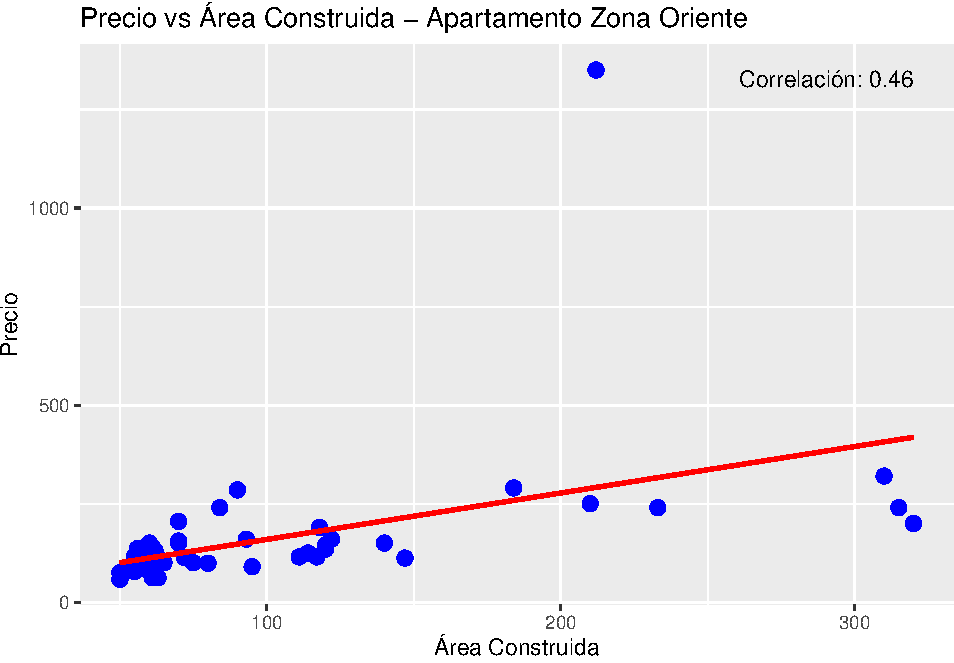
\includegraphics{A2_U2_InformeEjecutivo_files/figure-latex/unnamed-chunk-27-1.pdf}
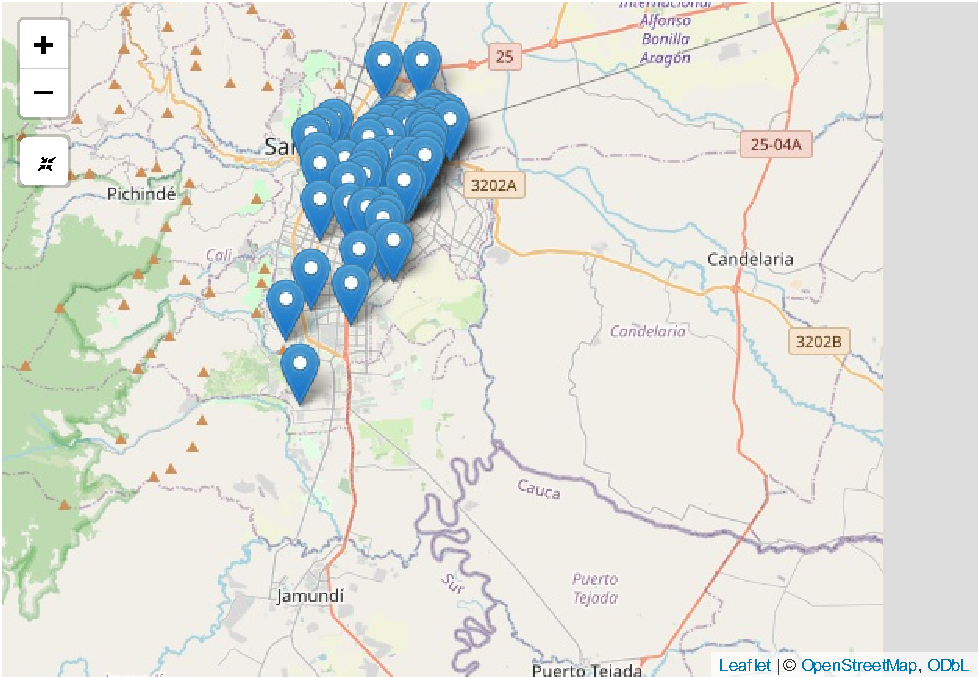
\includegraphics{A2_U2_InformeEjecutivo_files/figure-latex/unnamed-chunk-27-2.pdf}

\paragraph{\texorpdfstring{\textbf{Base 2 Apartamentos Zona
Centro}}{Base 2 Apartamentos Zona Centro}}\label{base-2-apartamentos-zona-centro}

\begin{verbatim}
## Primeros 3 registros de la base de datos filtrada:
\end{verbatim}

\begin{longtable}[]{@{}
  >{\raggedleft\arraybackslash}p{(\columnwidth - 24\tabcolsep) * \real{0.0420}}
  >{\raggedright\arraybackslash}p{(\columnwidth - 24\tabcolsep) * \real{0.1008}}
  >{\raggedright\arraybackslash}p{(\columnwidth - 24\tabcolsep) * \real{0.0420}}
  >{\raggedleft\arraybackslash}p{(\columnwidth - 24\tabcolsep) * \real{0.0672}}
  >{\raggedleft\arraybackslash}p{(\columnwidth - 24\tabcolsep) * \real{0.0672}}
  >{\raggedleft\arraybackslash}p{(\columnwidth - 24\tabcolsep) * \real{0.0840}}
  >{\raggedleft\arraybackslash}p{(\columnwidth - 24\tabcolsep) * \real{0.1092}}
  >{\raggedleft\arraybackslash}p{(\columnwidth - 24\tabcolsep) * \real{0.0588}}
  >{\raggedleft\arraybackslash}p{(\columnwidth - 24\tabcolsep) * \real{0.1092}}
  >{\raggedright\arraybackslash}p{(\columnwidth - 24\tabcolsep) * \real{0.1008}}
  >{\raggedright\arraybackslash}p{(\columnwidth - 24\tabcolsep) * \real{0.0672}}
  >{\raggedleft\arraybackslash}p{(\columnwidth - 24\tabcolsep) * \real{0.0840}}
  >{\raggedleft\arraybackslash}p{(\columnwidth - 24\tabcolsep) * \real{0.0672}}@{}}
\toprule\noalign{}
\begin{minipage}[b]{\linewidth}\raggedleft
id
\end{minipage} & \begin{minipage}[b]{\linewidth}\raggedright
zona
\end{minipage} & \begin{minipage}[b]{\linewidth}\raggedright
piso
\end{minipage} & \begin{minipage}[b]{\linewidth}\raggedleft
estrato
\end{minipage} & \begin{minipage}[b]{\linewidth}\raggedleft
preciom
\end{minipage} & \begin{minipage}[b]{\linewidth}\raggedleft
areaconst
\end{minipage} & \begin{minipage}[b]{\linewidth}\raggedleft
parqueaderos
\end{minipage} & \begin{minipage}[b]{\linewidth}\raggedleft
banios
\end{minipage} & \begin{minipage}[b]{\linewidth}\raggedleft
habitaciones
\end{minipage} & \begin{minipage}[b]{\linewidth}\raggedright
tipo
\end{minipage} & \begin{minipage}[b]{\linewidth}\raggedright
barrio
\end{minipage} & \begin{minipage}[b]{\linewidth}\raggedleft
longitud
\end{minipage} & \begin{minipage}[b]{\linewidth}\raggedleft
latitud
\end{minipage} \\
\midrule\noalign{}
\endhead
\bottomrule\noalign{}
\endlastfoot
4654 & Zona Centro & 03 & 3 & 100 & 70.00 & NA & 2 & 3 & Apartamento &
alameda & -76.53200 & 3.45200 \\
4408 & Zona Centro & 05 & 3 & 120 & 84.00 & 1 & 2 & 3 & Apartamento &
alameda & -76.53123 & 3.44011 \\
4395 & Zona Centro & 04 & 3 & 125 & 66.76 & NA & 2 & 3 & Apartamento &
bretaña & -76.53111 & 3.44034 \\
\end{longtable}

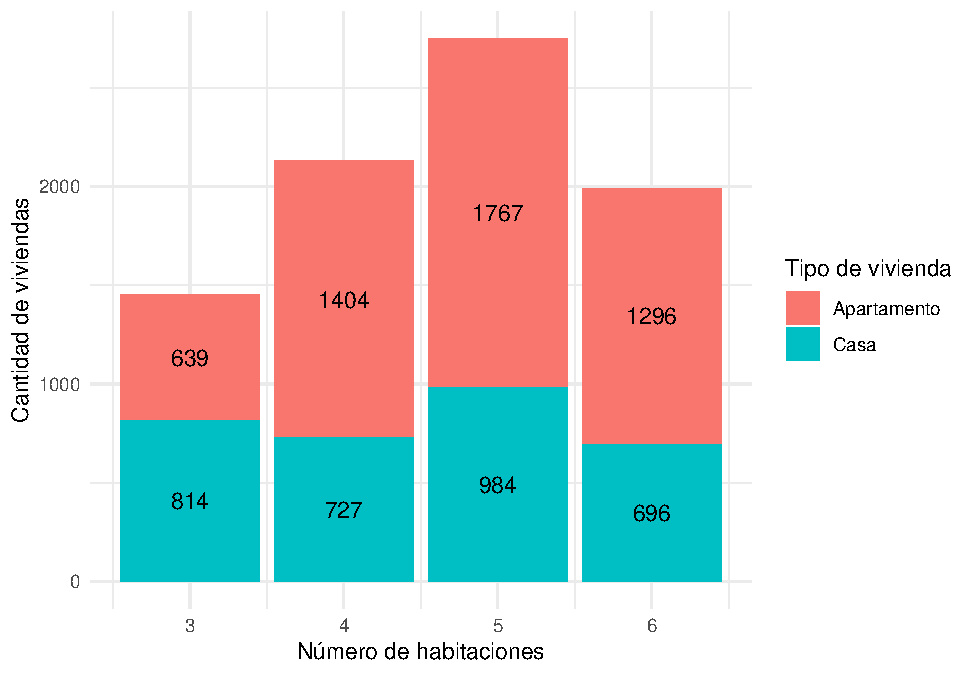
\includegraphics{A2_U2_InformeEjecutivo_files/figure-latex/unnamed-chunk-28-1.pdf}
\includegraphics{A2_U2_InformeEjecutivo_files/figure-latex/unnamed-chunk-28-2.pdf}

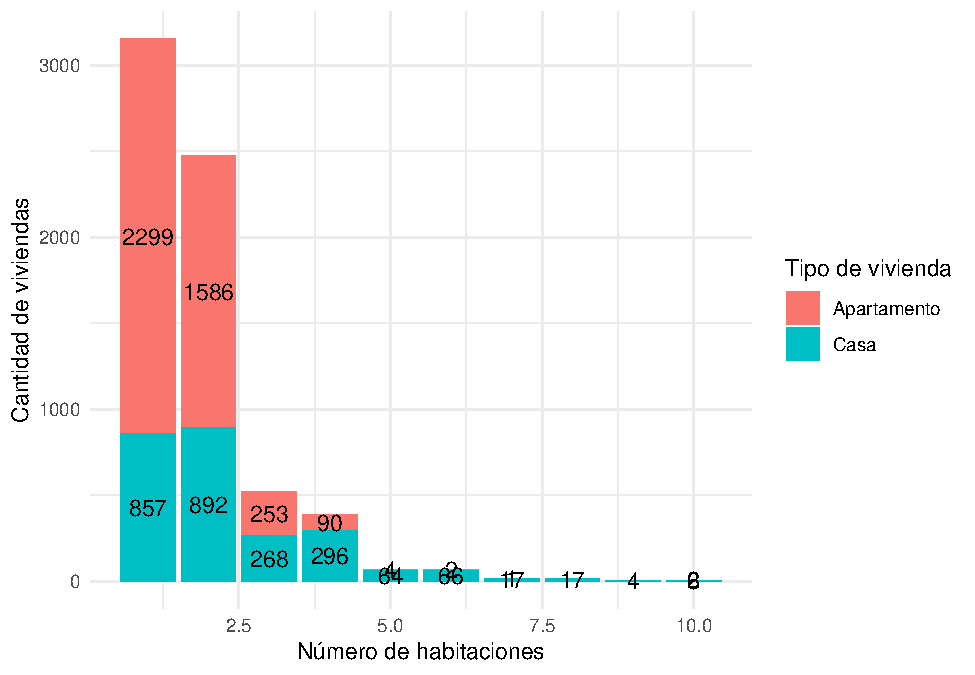
\includegraphics{A2_U2_InformeEjecutivo_files/figure-latex/unnamed-chunk-29-1.pdf}

\subparagraph{\texorpdfstring{\textbf{Análisis Comparativo por
Zonas}}{Análisis Comparativo por Zonas}}\label{anuxe1lisis-comparativo-por-zonas}

Basado en la información generada y el análisis del gráfico de
dispersión, se observan las siguientes tendencias:

\begin{itemize}
\tightlist
\item
  \textbf{Zona Oeste:}

  \begin{itemize}
  \tightlist
  \item
    Se aprecia la mayor concentración de puntos en la parte superior
    derecha del gráfico, lo que indica que esta zona tiene una elevada
    cantidad de propiedades con precios altos y amplias áreas
    construidas.\\
  \item
    Además, el rango de precios en la zona oeste es el más alto, y
    cuenta con el coeficiente de correlación más fuerte (0.82),
    sugiriendo una relación estrecha entre el precio y el área
    construida.
  \end{itemize}
\item
  \textbf{Zona Sur y Zona Norte:}

  \begin{itemize}
  \tightlist
  \item
    La Zona Sur presenta un coeficiente de correlación de 0.76, similar
    al de la Zona Norte, sin embargo, el rango de precios en la Zona Sur
    es ligeramente inferior.\\
  \item
    Aunque la Zona Norte tiene un rango de precios comparable al de la
    Zona Sur, se observa una menor concentración de puntos en la parte
    superior derecha del gráfico, lo que podría implicar una menor
    cantidad de propiedades con precios muy altos y áreas muy amplias.
  \end{itemize}
\item
  \textbf{Zona Oriente:}

  \begin{itemize}
  \tightlist
  \item
    Es la que muestra los precios más bajos en general.\\
  \item
    Aunque se detecta la presencia de un dato atípico en el gráfico,
    este no altera la tendencia general de precios bajos.
  \end{itemize}
\item
  \textbf{Zona Centro:}

  \begin{itemize}
  \tightlist
  \item
    Ofrece precios intermedios en comparación con las otras zonas.\\
  \item
    Se observa una menor oferta inmobiliaria de tipo apartamento, lo que
    podría estar relacionado con la dinámica comercial particular de
    esta área, favoreciendo un perfil de vivienda residencial diferente.
  \end{itemize}
\end{itemize}

Finalmente, es importante destacar que, al igual que se ha observado en
los datos del tipo de vivienda \textbf{\emph{``Casa''}}, se evidencia un
posible error humano en la asignación de la zona o en el registro de las
coordenadas (longitud y latitud). Esto se aprecia en el último gráfico,
donde se observan traslapos en los colores, especialmente en la parte
superior del mapa, lo que indic

\subsection{\texorpdfstring{\textbf{Analisis
exploratorio}}{Analisis exploratorio}}\label{analisis-exploratorio}

\begin{verbatim}
##        id           zona               piso              estrato     
##  Min.   :   3   Length:5100        Length:5100        Min.   :3.000  
##  1st Qu.:2180   Class :character   Class :character   1st Qu.:4.000  
##  Median :4158   Mode  :character   Mode  :character   Median :5.000  
##  Mean   :4284                                         Mean   :4.727  
##  3rd Qu.:6556                                         3rd Qu.:6.000  
##  Max.   :8317                                         Max.   :6.000  
##                                                                      
##     preciom         areaconst      parqueaderos        banios     
##  Min.   :  58.0   Min.   : 35.0   Min.   : 1.000   Min.   :0.000  
##  1st Qu.: 175.0   1st Qu.: 68.0   1st Qu.: 1.000   1st Qu.:2.000  
##  Median : 279.0   Median : 90.0   Median : 1.000   Median :2.000  
##  Mean   : 366.9   Mean   :112.8   Mean   : 1.568   Mean   :2.617  
##  3rd Qu.: 430.0   3rd Qu.:130.0   3rd Qu.: 2.000   3rd Qu.:3.000  
##  Max.   :1950.0   Max.   :932.0   Max.   :10.000   Max.   :8.000  
##                                   NA's   :869                     
##   habitaciones       tipo              barrio             longitud     
##  Min.   :0.000   Length:5100        Length:5100        Min.   :-76.59  
##  1st Qu.:3.000   Class :character   Class :character   1st Qu.:-76.54  
##  Median :3.000   Mode  :character   Mode  :character   Median :-76.53  
##  Mean   :2.971                                         Mean   :-76.53  
##  3rd Qu.:3.000                                         3rd Qu.:-76.52  
##  Max.   :9.000                                         Max.   :-76.46  
##                                                                        
##     latitud     
##  Min.   :3.334  
##  1st Qu.:3.380  
##  Median :3.419  
##  Mean   :3.419  
##  3rd Qu.:3.453  
##  Max.   :3.498  
## 
\end{verbatim}

\begin{verbatim}
## tibble [5,100 x 13] (S3: tbl_df/tbl/data.frame)
##  $ id          : num [1:5100] 1212 1724 2326 4386 7497 ...
##  $ zona        : chr [1:5100] "Zona Norte" "Zona Norte" "Zona Norte" "Zona Norte" ...
##  $ piso        : chr [1:5100] "01" "01" "01" "01" ...
##  $ estrato     : num [1:5100] 5 5 4 5 6 4 5 3 3 6 ...
##  $ preciom     : num [1:5100] 260 240 220 310 520 320 385 100 175 820 ...
##  $ areaconst   : num [1:5100] 90 87 52 137 98 108 103 49 80 377 ...
##  $ parqueaderos: num [1:5100] 1 1 2 2 2 2 2 NA 1 1 ...
##  $ banios      : num [1:5100] 2 3 2 3 2 3 2 1 2 4 ...
##  $ habitaciones: num [1:5100] 3 3 3 4 2 3 3 2 3 4 ...
##  $ tipo        : chr [1:5100] "Apartamento" "Apartamento" "Apartamento" "Apartamento" ...
##  $ barrio      : chr [1:5100] "acopi" "acopi" "acopi" "acopi" ...
##  $ longitud    : num [1:5100] -76.5 -76.5 -76.5 -76.5 -76.5 ...
##  $ latitud     : num [1:5100] 3.46 3.37 3.43 3.38 3.44 ...
\end{verbatim}

\begin{verbatim}
##        id          estrato         preciom         areaconst    
##  Min.   :   3   Min.   :3.000   Min.   :  58.0   Min.   : 35.0  
##  1st Qu.:2180   1st Qu.:4.000   1st Qu.: 175.0   1st Qu.: 68.0  
##  Median :4158   Median :5.000   Median : 279.0   Median : 90.0  
##  Mean   :4284   Mean   :4.727   Mean   : 366.9   Mean   :112.8  
##  3rd Qu.:6556   3rd Qu.:6.000   3rd Qu.: 430.0   3rd Qu.:130.0  
##  Max.   :8317   Max.   :6.000   Max.   :1950.0   Max.   :932.0  
##                                                                 
##   parqueaderos        banios       habitaciones      longitud     
##  Min.   : 1.000   Min.   :0.000   Min.   :0.000   Min.   :-76.59  
##  1st Qu.: 1.000   1st Qu.:2.000   1st Qu.:3.000   1st Qu.:-76.54  
##  Median : 1.000   Median :2.000   Median :3.000   Median :-76.53  
##  Mean   : 1.568   Mean   :2.617   Mean   :2.971   Mean   :-76.53  
##  3rd Qu.: 2.000   3rd Qu.:3.000   3rd Qu.:3.000   3rd Qu.:-76.52  
##  Max.   :10.000   Max.   :8.000   Max.   :9.000   Max.   :-76.46  
##  NA's   :869                                                      
##     latitud     
##  Min.   :3.334  
##  1st Qu.:3.380  
##  Median :3.419  
##  Mean   :3.419  
##  3rd Qu.:3.453  
##  Max.   :3.498  
## 
\end{verbatim}

\begin{verbatim}
## < table of extent 0 x 0 >
\end{verbatim}

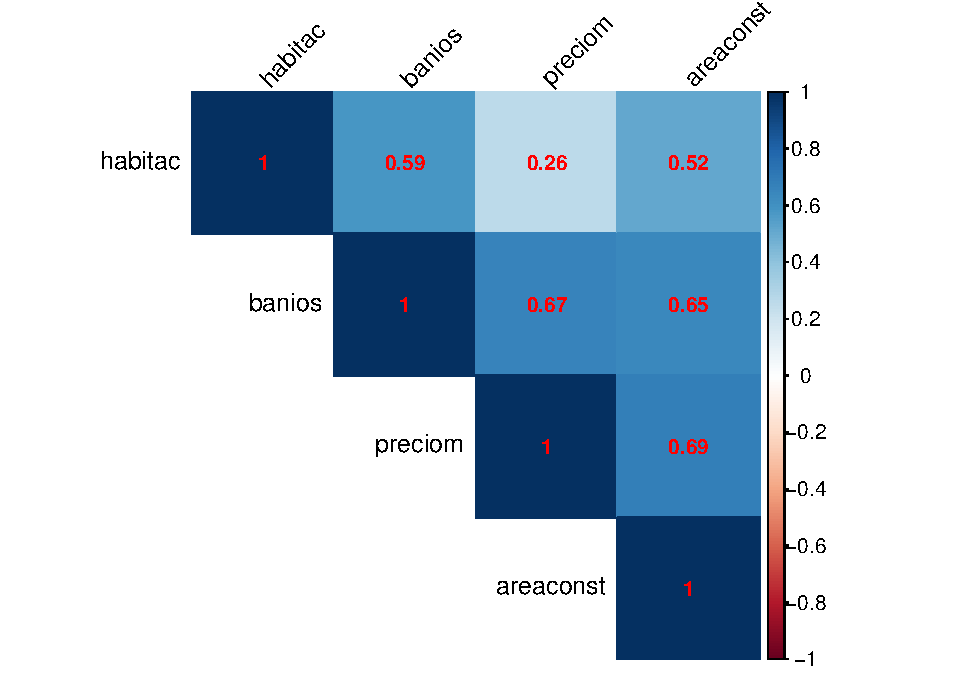
\includegraphics{A2_U2_InformeEjecutivo_files/figure-latex/unnamed-chunk-31-1.pdf}
\includegraphics{A2_U2_InformeEjecutivo_files/figure-latex/unnamed-chunk-31-2.pdf}

\begin{verbatim}
## $preciom
##               Df    Sum Sq  Mean Sq F value Pr(>F)    
## zona           4 118380819 29595205   489.3 <2e-16 ***
## Residuals   5095 308139573    60479                   
## ---
## Signif. codes:  0 '***' 0.001 '**' 0.01 '*' 0.05 '.' 0.1 ' ' 1
## 
## $areaconst
##               Df   Sum Sq Mean Sq F value Pr(>F)    
## zona           4  4566161 1141540   291.3 <2e-16 ***
## Residuals   5095 19963328    3918                   
## ---
## Signif. codes:  0 '***' 0.001 '**' 0.01 '*' 0.05 '.' 0.1 ' ' 1
## 
## $estrato
##               Df Sum Sq Mean Sq F value Pr(>F)    
## zona           4   1156  289.03   396.3 <2e-16 ***
## Residuals   5095   3715    0.73                   
## ---
## Signif. codes:  0 '***' 0.001 '**' 0.01 '*' 0.05 '.' 0.1 ' ' 1
## 
## $banios
##               Df Sum Sq Mean Sq F value Pr(>F)    
## zona           4    827  206.79   210.9 <2e-16 ***
## Residuals   5095   4996    0.98                   
## ---
## Signif. codes:  0 '***' 0.001 '**' 0.01 '*' 0.05 '.' 0.1 ' ' 1
## 
## $habitaciones
##               Df Sum Sq Mean Sq F value   Pr(>F)    
## zona           4     18   4.508   9.935 5.25e-08 ***
## Residuals   5095   2312   0.454                     
## ---
## Signif. codes:  0 '***' 0.001 '**' 0.01 '*' 0.05 '.' 0.1 ' ' 1
\end{verbatim}

\begin{longtable}[]{@{}ll@{}}
\caption{Data summary}\tabularnewline
\toprule\noalign{}
\endfirsthead
\endhead
\bottomrule\noalign{}
\endlastfoot
Name & vivienda\_apartamento \\
Number of rows & 5100 \\
Number of columns & 13 \\
\_\_\_\_\_\_\_\_\_\_\_\_\_\_\_\_\_\_\_\_\_\_\_ & \\
Column type frequency: & \\
character & 4 \\
numeric & 9 \\
\_\_\_\_\_\_\_\_\_\_\_\_\_\_\_\_\_\_\_\_\_\_\_\_ & \\
Group variables & None \\
\end{longtable}

\textbf{Variable type: character}

\begin{longtable}[]{@{}
  >{\raggedright\arraybackslash}p{(\columnwidth - 14\tabcolsep) * \real{0.1944}}
  >{\raggedleft\arraybackslash}p{(\columnwidth - 14\tabcolsep) * \real{0.1389}}
  >{\raggedleft\arraybackslash}p{(\columnwidth - 14\tabcolsep) * \real{0.1944}}
  >{\raggedleft\arraybackslash}p{(\columnwidth - 14\tabcolsep) * \real{0.0556}}
  >{\raggedleft\arraybackslash}p{(\columnwidth - 14\tabcolsep) * \real{0.0556}}
  >{\raggedleft\arraybackslash}p{(\columnwidth - 14\tabcolsep) * \real{0.0833}}
  >{\raggedleft\arraybackslash}p{(\columnwidth - 14\tabcolsep) * \real{0.1250}}
  >{\raggedleft\arraybackslash}p{(\columnwidth - 14\tabcolsep) * \real{0.1528}}@{}}
\toprule\noalign{}
\begin{minipage}[b]{\linewidth}\raggedright
skim\_variable
\end{minipage} & \begin{minipage}[b]{\linewidth}\raggedleft
n\_missing
\end{minipage} & \begin{minipage}[b]{\linewidth}\raggedleft
complete\_rate
\end{minipage} & \begin{minipage}[b]{\linewidth}\raggedleft
min
\end{minipage} & \begin{minipage}[b]{\linewidth}\raggedleft
max
\end{minipage} & \begin{minipage}[b]{\linewidth}\raggedleft
empty
\end{minipage} & \begin{minipage}[b]{\linewidth}\raggedleft
n\_unique
\end{minipage} & \begin{minipage}[b]{\linewidth}\raggedleft
whitespace
\end{minipage} \\
\midrule\noalign{}
\endhead
\bottomrule\noalign{}
\endlastfoot
zona & 0 & 1.00 & 8 & 12 & 0 & 5 & 0 \\
piso & 1381 & 0.73 & 2 & 2 & 0 & 12 & 0 \\
tipo & 0 & 1.00 & 11 & 11 & 0 & 1 & 0 \\
barrio & 0 & 1.00 & 4 & 29 & 0 & 289 & 0 \\
\end{longtable}

\textbf{Variable type: numeric}

\begin{longtable}[]{@{}
  >{\raggedright\arraybackslash}p{(\columnwidth - 20\tabcolsep) * \real{0.1414}}
  >{\raggedleft\arraybackslash}p{(\columnwidth - 20\tabcolsep) * \real{0.1010}}
  >{\raggedleft\arraybackslash}p{(\columnwidth - 20\tabcolsep) * \real{0.1414}}
  >{\raggedleft\arraybackslash}p{(\columnwidth - 20\tabcolsep) * \real{0.0808}}
  >{\raggedleft\arraybackslash}p{(\columnwidth - 20\tabcolsep) * \real{0.0808}}
  >{\raggedleft\arraybackslash}p{(\columnwidth - 20\tabcolsep) * \real{0.0707}}
  >{\raggedleft\arraybackslash}p{(\columnwidth - 20\tabcolsep) * \real{0.0808}}
  >{\raggedleft\arraybackslash}p{(\columnwidth - 20\tabcolsep) * \real{0.0808}}
  >{\raggedleft\arraybackslash}p{(\columnwidth - 20\tabcolsep) * \real{0.0808}}
  >{\raggedleft\arraybackslash}p{(\columnwidth - 20\tabcolsep) * \real{0.0808}}
  >{\raggedright\arraybackslash}p{(\columnwidth - 20\tabcolsep) * \real{0.0606}}@{}}
\toprule\noalign{}
\begin{minipage}[b]{\linewidth}\raggedright
skim\_variable
\end{minipage} & \begin{minipage}[b]{\linewidth}\raggedleft
n\_missing
\end{minipage} & \begin{minipage}[b]{\linewidth}\raggedleft
complete\_rate
\end{minipage} & \begin{minipage}[b]{\linewidth}\raggedleft
mean
\end{minipage} & \begin{minipage}[b]{\linewidth}\raggedleft
sd
\end{minipage} & \begin{minipage}[b]{\linewidth}\raggedleft
p0
\end{minipage} & \begin{minipage}[b]{\linewidth}\raggedleft
p25
\end{minipage} & \begin{minipage}[b]{\linewidth}\raggedleft
p50
\end{minipage} & \begin{minipage}[b]{\linewidth}\raggedleft
p75
\end{minipage} & \begin{minipage}[b]{\linewidth}\raggedleft
p100
\end{minipage} & \begin{minipage}[b]{\linewidth}\raggedright
hist
\end{minipage} \\
\midrule\noalign{}
\endhead
\bottomrule\noalign{}
\endlastfoot
id & 0 & 1.00 & 4284.03 & 2449.82 & 3.00 & 2179.75 & 4158.50 & 6556.25 &
8317.00 & ▆▇▆▆▇ \\
estrato & 0 & 1.00 & 4.73 & 0.98 & 3.00 & 4.00 & 5.00 & 6.00 & 6.00 &
▃▆▁▇▆ \\
preciom & 0 & 1.00 & 366.94 & 289.22 & 58.00 & 175.00 & 279.00 & 430.00
& 1950.00 & ▇▂▁▁▁ \\
areaconst & 0 & 1.00 & 112.78 & 69.36 & 35.00 & 68.00 & 90.00 & 130.00 &
932.00 & ▇▁▁▁▁ \\
parqueaderos & 869 & 0.83 & 1.57 & 0.74 & 1.00 & 1.00 & 1.00 & 2.00 &
10.00 & ▇▁▁▁▁ \\
banios & 0 & 1.00 & 2.62 & 1.07 & 0.00 & 2.00 & 2.00 & 3.00 & 8.00 &
▁▇▂▁▁ \\
habitaciones & 0 & 1.00 & 2.97 & 0.68 & 0.00 & 3.00 & 3.00 & 3.00 & 9.00
& ▁▇▂▁▁ \\
longitud & 0 & 1.00 & -76.53 & 0.02 & -76.59 & -76.54 & -76.53 & -76.52
& -76.46 & ▁▅▇▂▁ \\
latitud & 0 & 1.00 & 3.42 & 0.04 & 3.33 & 3.38 & 3.42 & 3.45 & 3.50 &
▂▇▅▇▅ \\
\end{longtable}

\paragraph{\texorpdfstring{\textbf{Interpretación del
Modelo}}{Interpretación del Modelo}}\label{interpretaciuxf3n-del-modelo}

El modelo de regresión lineal múltiple ajustado se expresa de la
siguiente manera:

\[
\text{Precio} = \beta_0 + \beta_1 \times \text{Área Construida} + \beta_2 \times \text{Estrato} + \beta_3 \times \text{Parqueaderos} + \beta_4 \times \text{Baños} + \beta_5 \times \text{Habitaciones} + \varepsilon
\]

Donde:

\begin{itemize}
\tightlist
\item
  \textbf{\(\beta_0\) (Intercepto):} Representa el precio estimado
  cuando todas las variables independientes son cero.
\item
  \textbf{\(\beta_1, \beta_2, \beta_3, \beta_4, \beta_5\) (Coeficientes
  de Regresión):} Cada uno de estos coeficientes indica el cambio
  esperado en el precio ante un incremento unitario en la variable
  correspondiente, manteniendo constantes las demás variables.
\item
  \textbf{\(\varepsilon\) (Término de Error):} Captura la variabilidad
  en el precio que no es explicada por el modelo.
\end{itemize}

Este modelo permite estimar el precio de una vivienda basándose en sus
características, tales como el área construida, el estrato, el número de
parqueaderos, baños y habitaciones.

\begin{verbatim}
## 
## Call:
## lm(formula = preciom ~ areaconst + estrato + banios + habitaciones + 
##     zona, data = vivienda_apartamento_seleccion)
## 
## Residuals:
##      Min       1Q   Median       3Q      Max 
## -1904.61   -51.00     1.05    45.20   971.19 
## 
## Coefficients:
##                    Estimate Std. Error t value Pr(>|t|)    
## (Intercept)      -257.42194   29.85912  -8.621  < 2e-16 ***
## areaconst           2.22296    0.04204  52.873  < 2e-16 ***
## estrato            56.91854    2.68697  21.183  < 2e-16 ***
## banios             61.11292    2.99576  20.400  < 2e-16 ***
## habitaciones      -32.93022    3.32925  -9.891  < 2e-16 ***
## zonaZona Norte     31.08865   27.80772   1.118    0.264    
## zonaZona Oeste    118.86179   28.15735   4.221 2.47e-05 ***
## zonaZona Oriente   19.31989   32.37714   0.597    0.551    
## zonaZona Sur       20.09085   27.71277   0.725    0.469    
## ---
## Signif. codes:  0 '***' 0.001 '**' 0.01 '*' 0.05 '.' 0.1 ' ' 1
## 
## Residual standard error: 134.6 on 5091 degrees of freedom
## Multiple R-squared:  0.7839, Adjusted R-squared:  0.7836 
## F-statistic:  2308 on 8 and 5091 DF,  p-value: < 2.2e-16
\end{verbatim}

\begin{verbatim}
## El coeficiente para el área construida es: 2.222963
\end{verbatim}

\begin{verbatim}
## Los coeficientes para los estratos son: 56.91854
\end{verbatim}

\begin{verbatim}
## El coeficiente para los baños es: 61.11292
\end{verbatim}

\begin{verbatim}
## El coeficiente para las habitaciones es: -32.93022
\end{verbatim}

\begin{verbatim}
## Los coeficientes para las zonas son: 31.08865 118.8618 19.31989 20.09085
\end{verbatim}

\begin{verbatim}
## El R^2 del modelo es: 0.7838911
\end{verbatim}

El análisis del modelo de regresión aplicado revela que el precio de la
vivienda está fuertemente influenciado por diversas características. A
continuación se presentan los hallazgos principales:

\begin{itemize}
\item
  \textbf{Área Construida:}\\
  Cada metro cuadrado adicional en el área construida se asocia con un
  incremento aproximado de \textbf{\$2.22 millones} en el precio de la
  vivienda.
\item
  \textbf{Estrato:}\\
  Los estratos tienen un impacto significativo en el precio. En
  particular, para el estrato 6 se observa un aumento de aproximadamente
  \textbf{\$56.92 millones} por unidad, lo que sugiere que las viviendas
  en este nivel socioeconómico tienden a tener precios más elevados.
\item
  \textbf{Baños y Habitaciones:}

  \begin{itemize}
  \tightlist
  \item
    Cada baño adicional se asocia con un aumento de alrededor de
    \textbf{\$61.11 millones} en el precio.\\
  \item
    Por el contrario, cada habitación adicional se relaciona con una
    disminución de cerca de \textbf{\$32.93 millones}, lo cual podría
    reflejar efectos complejos en la distribución de espacios o en la
    valoración del inmueble.
  \end{itemize}
\item
  \textbf{Zonas:}\\
  Las variaciones de precios según la zona son notables:

  \begin{itemize}
  \tightlist
  \item
    \textbf{Zona Sur:} Presenta el mayor impacto, incrementando el
    precio en aproximadamente \textbf{\$118.86 millones}.
  \item
    \textbf{Zona Norte:} Contribuye con un aumento de alrededor de
    \textbf{\$31.09 millones}.
  \item
    \textbf{Zona Oeste:} Se asocia con un incremento de cerca de
    \textbf{\$20.09 millones}.
  \item
    \textbf{Zona Centro:} Aporta un aumento aproximado de
    \textbf{\$19.32 millones}.
  \end{itemize}
\end{itemize}

Finalmente, el modelo cuenta con un coeficiente de determinación
(\textbf{R²}) de aproximadamente \textbf{0.78}, lo que significa que
cerca del \textbf{78.39\%} de la variabilidad en el precio de la
vivienda es explicada por las variables incluidas en el modelo, lo que
demuestra un buen ajuste.

\subsection{\texorpdfstring{\textbf{Validacion de
supuestos}}{Validacion de supuestos}}\label{validacion-de-supuestos}

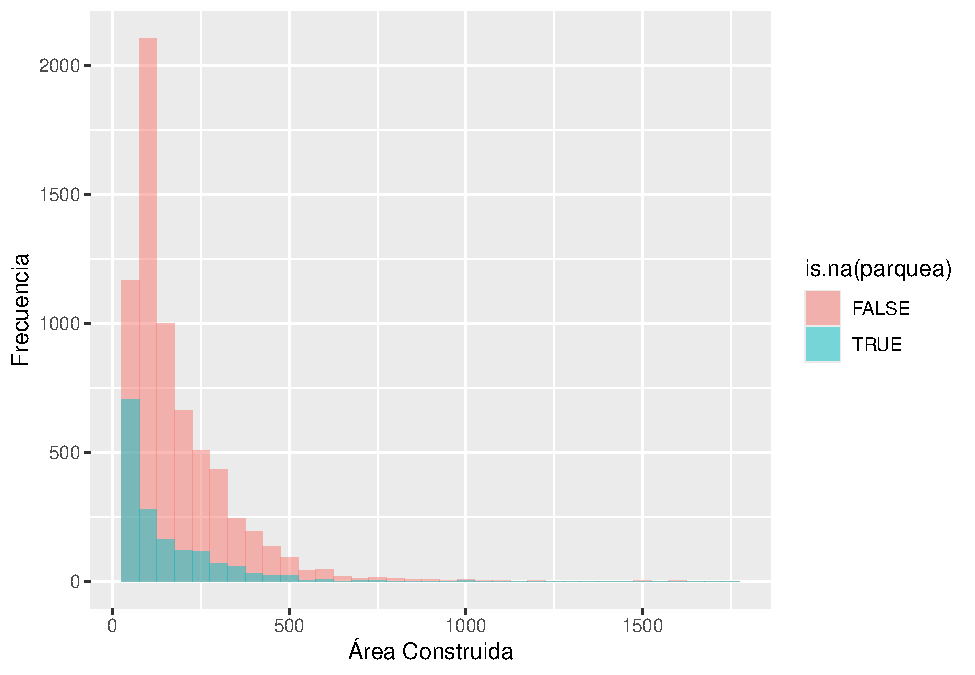
\includegraphics{A2_U2_InformeEjecutivo_files/figure-latex/unnamed-chunk-33-1.pdf}
\includegraphics{A2_U2_InformeEjecutivo_files/figure-latex/unnamed-chunk-33-2.pdf}

\begin{verbatim}
## 
##  studentized Breusch-Pagan test
## 
## data:  modelo_regresion
## BP = 1465.5, df = 8, p-value < 2.2e-16
\end{verbatim}

\begin{verbatim}
## 
##  Box-Ljung test
## 
## data:  modelo_regresion$resid
## X-squared = 127.18, df = 1, p-value < 2.2e-16
\end{verbatim}

\textbf{Test de Breusch-Pagan para Homocedasticidad:}

\begin{itemize}
\tightlist
\item
  \textbf{Estadístico de prueba (BP):} 1465.5 con 8 grados de libertad.
\item
  \textbf{p-valor:} \textless{} 2.2e-16.
\end{itemize}

El resultado significativo (p \textless{} 2.2e-16) indica que se rechaza
la hipótesis nula de homocedasticidad, sugiriendo que los residuos del
modelo no tienen una varianza constante.

\textbf{Test de Ljung-Box para Autocorrelación de los Residuos:}

\begin{itemize}
\tightlist
\item
  \textbf{Estadístico de prueba (X-squared):} 127.18 con 1 grado de
  libertad.
\item
  \textbf{p-valor:} \textless{} 2.2e-16.
\end{itemize}

El bajo \textbf{p-valor} respalda el rechazo de la hipótesis nula de
independencia de los residuos, indicando que éstos presentan
autocorrelación. Ambos tests evidencian que el modelo de regresión
lineal múltiple no cumple completamente con los supuestos de
homocedasticidad e independencia de los residuos, lo que podría afectar
la precisión de las estimaciones y las pruebas de hipótesis derivadas
del modelo.

\subsection{\texorpdfstring{\textbf{Predicción del
precio}}{Predicción del precio}}\label{predicciuxf3n-del-precio}

\begin{verbatim}
##        1        2 
## 732.8381 789.7567
\end{verbatim}

La predicción del precio para la vivienda varía según el estrato
considerado. Es decir, para una vivienda ubicada en estrato 5, se estima
un precio aproximado de \textbf{\$732.84 millones}, mientras que para
una en estrato 6, el precio predicho asciende a alrededor de
\textbf{\$789.76 millones}.

\subsection{\texorpdfstring{\textbf{Potenciales
ofertas}}{Potenciales ofertas}}\label{potenciales-ofertas}

\begin{verbatim}
##   areaconst banios habitaciones estrato     zona precio_estimado
## 1       280      3            4       5 Zona Sur        721.3091
## 2       300      3            4       5 Zona Sur        765.7684
## 3       280      4            4       5 Zona Sur        782.4220
## 4       300      4            4       5 Zona Sur        826.8813
## 5       280      3            5       5 Zona Sur        688.3789
\end{verbatim}

Las ofertas potenciales brindan una diversidad de opciones en cuanto a
tamaño, distribución de espacios y precios. A continuación se describen
detalladamente las características de cada una de las cinco ofertas
identificadas:

\begin{enumerate}
\def\labelenumi{\arabic{enumi}.}
\item
  \textbf{Primera Oferta:}\\
  Esta opción ofrece una vivienda con un área construida de 280 m², que
  incluye 3 baños y 4 habitaciones. Con un precio estimado de
  aproximadamente \$721.31 millones, representa un equilibrio atractivo
  entre dimensiones y costo.
\item
  \textbf{Segunda Oferta:}\\
  Con un área de 300 m², esta opción mantiene 3 baños y 4 habitaciones,
  pero su precio es ligeramente superior, alrededor de \$765.77
  millones. La diferencia en precio podría reflejar mejoras en el diseño
  o acabados que aporten mayor valor.
\item
  \textbf{Tercera Oferta:}\\
  Esta alternativa cuenta con 280 m² de área construida y una
  configuración que incluye 4 baños y 4 habitaciones, situándose en un
  rango de precio de aproximadamente \$782.42 millones. La adición de un
  baño extra puede ser un factor diferenciador para quienes buscan mayor
  funcionalidad.
\item
  \textbf{Cuarta Oferta:}\\
  Con un área de 300 m², 4 baños y 4 habitaciones, esta opción se
  posiciona en el rango de precio más alto, estimado en cerca de
  \$826.88 millones. Es ideal para compradores que priorizan espacios
  amplios y mayores comodidades.
\item
  \textbf{Quinta Oferta:}\\
  Esta oferta, con 280 m² de área construida, se distingue por contar
  con 3 baños y 5 habitaciones, ofreciendo el precio más competitivo,
  alrededor de \$688.38 millones. La mayor cantidad de habitaciones a un
  costo inferior la convierte en una alternativa especialmente atractiva
  para optimizar el uso del espacio sin exceder el presupuesto.
\end{enumerate}

\subsection{\texorpdfstring{\textbf{8. Anexos - Repositorio Código
fuente}}{8. Anexos - Repositorio Código fuente}}\label{anexos---repositorio-cuxf3digo-fuente}

Repositorio Github

\end{document}
